%%%%%%%%%%%%%%%%%%%%%%%%%%%%%%%%%%%%%%%
\section{\label{sec:DAGMan}DAGMan Applications}
%%%%%%%%%%%%%%%%%%%%%%%%%%%%%%%%%%%%%%%
\index{DAGMan|(}
\index{directed acyclic graph (DAG)}
\index{Directed Acyclic Graph Manager (DAGMan)}
\index{job!dependencies within}

A directed acyclic graph (DAG) can be used to represent a set of computations
where the input, output, or execution of one or more computations
is dependent on one or more other computations.
The computations are nodes (vertices) in the graph,
and the edges (arcs) identify the dependencies.
HTCondor finds machines for the execution of programs, but it
does not schedule programs based on dependencies.
The Directed Acyclic Graph Manager (DAGMan) is a meta-scheduler for 
the execution of programs (computations). 
DAGMan submits the programs to HTCondor in an order represented by
a DAG and processes the results.
A \Term{DAG input file} describes the DAG.

DAGMan is itself executed as a scheduler universe job
within HTCondor.
It submits the HTCondor jobs within nodes in such a way as to
enforce the DAG's dependencies.
DAGMan also handles recovery and reporting
on the HTCondor jobs.

%%%%%%%%%%%%%%%%%%%%%%%%%%%%%%%%%%%%%%%
\subsection{\label{sec:DAGTerminology}DAGMan Terminology}
%%%%%%%%%%%%%%%%%%%%%%%%%%%%%%%%%%%%%%%
\index{DAGMan!terminology}

A node within a DAG may encompass more than a single
program submitted to run under HTCondor.
Figure~\ref{fig:dagman-node} illustrates the elements of a node.

\begin{figure}[hbt]
\centering
\includegraphics{user-man/dagman-node.eps}
\caption{\label{fig:dagman-node}One Node within a DAG}
\end{figure}

More than one HTCondor job may belong to a single node.
All HTCondor jobs within a node must be within
a single cluster, as given by the job ClassAd attribute \Attr{ClusterId}.
%In addition,
%all jobs within the single cluster must use the same log file.
%Separate nodes within a DAG may use different log files.

\emph{DAGMan enforces the dependencies within a DAG
using the events recorded in a separate
file that is specified by the default configuration.
If the exact same DAG were to be submitted more than once,
such that these DAGs were running at the same time,
expected them to fail in unpredictable and unexpected ways.
They would all be using the same single file to enforce dependencies. }

As DAGMan schedules and submits jobs within nodes to HTCondor,
these jobs are defined to succeed or fail based on their
return values.
This success or failure is propagated in well-defined ways to the level of
a node within a DAG.
Further progression of computation
(towards completing the DAG)
is based upon the success or failure of nodes.

The failure of a single job within a cluster
of multiple jobs
(within a single node)
causes the entire cluster of jobs to fail.
Any other jobs within the failed cluster of jobs are
immediately removed.
Each node within a DAG may be further constrained  to succeed or fail
based upon the return values of a PRE script and/or a POST script.

%%%%%%%%%%%%%%%%%%%%%%%%%%%%%%%%%%%%%%%
\subsection{The DAG Input File: Basic Commands}
%%%%%%%%%%%%%%%%%%%%%%%%%%%%%%%%%%%%%%%
\index{DAGMan!DAG input file}

The input file used by DAGMan is called a DAG input file.
It specifies the nodes of the DAG as well as the dependencies
that order the DAG.
All items are optional, except that there must be at least one \Arg{JOB}
item.

Comments may be placed in the DAG input file.
The pound character (\verb@#@) as the first character on a
line identifies the line as a comment.
Comments do not span lines.

A simple diamond-shaped DAG, as shown in
Figure~\ref{fig:dagman-diamond}
is presented as a starting point for examples.
This DAG contains 4 nodes.

\begin{figure}[hbt]
\centering
\includegraphics{user-man/dagman-diamond.eps}
\caption{\label{fig:dagman-diamond}Diamond DAG}
\end{figure}


A very simple DAG input file for this diamond-shaped DAG is

\footnotesize
\begin{verbatim}
    # File name: diamond.dag
    #
    JOB  A  A.condor 
    JOB  B  B.condor 
    JOB  C  C.condor	
    JOB  D  D.condor
    PARENT A CHILD B C
    PARENT B C CHILD D
\end{verbatim}
\normalsize

A set of basic commands appearing in a DAG input file is described below.


%%%%%%%%%%%%%%%%%%%%%%%%%%%%%%%%%%%%%%%
\subsubsection{\label{sec:dagman_job_command}JOB}
\label{dagman:JOB}
\index{DAG input file!JOB command}

The \Arg{JOB} command specifies an HTCondor job.
The syntax used for each \Arg{JOB} entry is

\Opt{JOB} \Arg{JobName} \Arg{SubmitDescriptionFileName}
\oOptArg{DIR}{directory} \oOpt{NOOP} \oOpt{DONE}

A \Arg{JOB} entry maps a \Arg{JobName} to an HTCondor submit description file.
The \Arg{JobName} uniquely identifies nodes within the
DAG input file and in output messages.
Each node name, given by \Arg{JobName}, within the DAG must be unique.
The \Arg{JOB} entry must appear within the DAG input file before
other items that reference the node.

The keywords \Arg{JOB}, \Arg{DIR}, \Arg{NOOP}, and \Arg{DONE}
are not case sensitive.
Therefore, \Arg{DONE}, \Arg{Done}, and \Arg{done} are all equivalent.
The values defined for \Arg{JobName} and \Arg{SubmitDescriptionFileName}
are case sensitive, as file names 
in a file system are case sensitive.
The \Arg{JobName} can be any string that contains no white space, except
for the strings \Arg{PARENT} and \Arg{CHILD} (in upper, lower, or mixed
case).

Note that \Arg{DIR}, \Arg{NOOP}, and \Arg{DONE}, if used, must appear
in the order shown above.

The optional \Arg{DIR} keyword specifies a working directory
for this node,
from which the HTCondor job will be submitted,
and from which a \Arg{PRE} and/or
\Arg{POST} script will be run.
If a relative directory is specified, it is relative to the current working 
directory as the DAG is submitted.
Note that a DAG containing \Arg{DIR} specifications cannot
be run in conjunction with the \Arg{-usedagdir} command-line
argument to \Condor{submit\_dag}.  A Rescue DAG generated by
a DAG run with the \Arg{-usedagdir} argument will contain
\Arg{DIR} specifications, so the \Arg{-usedagdir} argument is
automatically disregarded when running a Rescue DAG.

\label{dagman:NOOP}
The optional \Arg{NOOP} keyword identifies that the HTCondor job within
the node is not to be submitted to HTCondor.
This optimization is useful in cases such as debugging a complex DAG structure,
where some of the individual jobs are long-running.
For this debugging of structure,
some jobs are marked as \Arg{NOOP}s, and
the DAG is initially run to verify that the control flow through
the DAG is correct.
The \Arg{NOOP} keywords are then removed before submitting the DAG.
Any PRE and POST scripts
for jobs specified with \Arg{NOOP} \emph{are} executed;
to avoid running the PRE and POST scripts, comment them out.
The job that is not submitted to HTCondor is given a return value that indicates
success, such that the node may also succeed.
Return values of any 
PRE and POST scripts may still cause the node to fail.
Even though the job specified with \Arg{NOOP} is not submitted,
its submit description file must exist;
the log file for the job is used, 
because DAGMan generates dummy submission and termination events for the job.

The optional \Arg{DONE} keyword identifies a node as being already
completed.
This is mainly used by Rescue DAGs generated by DAGMan itself,
in the event of a failure to complete the workflow.
Nodes with the \Arg{DONE} keyword are not executed when the Rescue DAG is run,
allowing the workflow to pick up from the previous endpoint.  Users
should generally not use the \Arg{DONE} keyword.
The \Arg{NOOP} keyword is more flexible in avoiding
the execution of a job within a node.
Note that, for any node marked \Arg{DONE} in a DAG, all of
its parents must also be marked \Arg{DONE}; 
otherwise, a fatal error will result.
The \Arg{DONE} keyword applies to the entire node.
A node marked with \Arg{DONE} will not have a PRE or POST script run,
and the HTCondor job will not be submitted.

%%%%%%%%%%%%%%%%%%%%%%%%%%%%%%%%%%%%%%%
\subsubsection{\label{sec:dagman_data_command}DATA}
\label{dagman:DATA}
\index{DAG input file!DATA command}

As of version 8.3.5, \Condor{dagman} no longer supports DATA nodes.

%%%%%%%%%%%%%%%%%%%%%%%%%%%%%%%%%%%%%%%
\subsubsection{\label{sec:dagman_parent_child_command}PARENT \Dots CHILD}
\label{dagman:ParentChild}
\index{DAG input file!PARENT \Dots CHILD command}

The \Arg{PARENT} \Arg{CHILD} command specifies the
dependencies within the DAG.
\index{DAGMan!describing dependencies}
Nodes are parents and/or children within the DAG.
A parent node must be completed successfully before
any of its children may be started.
A child node may only be started once
all its parents have successfully completed.

The syntax used for each dependency entry is

\Opt{PARENT} \Arg{ParentJobName\Dots} \Opt{CHILD} \Arg{ChildJobName\Dots}

The \Arg{PARENT} keyword is followed by one or more
\Arg{ParentJobName}s.
The \Arg{CHILD} keyword is followed by one or more
\Arg{ChildJobName}s.
Each child job depends on every parent job within the line.
A single line in the input file can specify the dependencies from one or more
parents to one or more children.
The diamond-shaped DAG example may specify the dependencies with
\begin{verbatim}
PARENT A CHILD B C
PARENT B C CHILD D
\end{verbatim}
An alternative specification for the diamond-shaped DAG
may specify some or all of the dependencies on separate lines:
\begin{verbatim}
PARENT A CHILD B C
PARENT B CHILD D
PARENT C CHILD D
\end{verbatim}

As a further example, the line
\begin{verbatim}
PARENT p1 p2 CHILD c1 c2
\end{verbatim}
produces four dependencies:
\begin{enumerate}
\item{\verb@p1@ to \verb@c1@}
\item{\verb@p1@ to \verb@c2@}
\item{\verb@p2@ to \verb@c1@}
\item{\verb@p2@ to \verb@c2@}
\end{enumerate}

%%%%%%%%%%%%%%%%%%%%%%%%%%%%%%%%%%%%%%%
\subsubsection{\label{sec:dagman_script_command}SCRIPT}
\label{dagman:SCRIPT}
\index{DAG input file!SCRIPT command}
\index{DAGMan!PRE and POST scripts}

The optional \Arg{SCRIPT} command specifies
processing that is done either before a job within
a node is submitted
or after a job within a node completes its execution.
\index{DAGMan!PRE script}
Processing done before a job is submitted is
called a \Arg{PRE} script.
Processing done after a job completes its execution is
\index{DAGMan!POST script}
called a \Arg{POST} script.
Note that the executable specified does not necessarily
have to be a shell script (Unix) or batch file (Windows);
but it should be relatively light weight because it will
be run directly on the submit machine, not submitted as
an HTCondor job.

The syntax used for each \Arg{PRE} or \Arg{POST} entry is

\Opt{SCRIPT} \oOptArg{DEFER}{status time}
\Opt{PRE} \Arg{JobName} \Arg{ExecutableName} \oArg{arguments}

\Opt{SCRIPT} \oOptArg{DEFER}{status time}
\Opt{POST}  \Arg{JobName} \Arg{ExecutableName} \oArg{arguments}

The \Arg{SCRIPT} command uses
the \Arg{PRE} or \Arg{POST} keyword,
which specifies the relative timing of when the script is to be run.
The \Arg{JobName} identifies the node to which the script is attached.
The \Arg{ExecutableName}
specifies the executable (e.g., shell script or batch file) to be executed, 
and may not contain spaces.
The optional \Arg{arguments} are command line arguments to the script,
and spaces delimit the arguments.
Both \Arg{ExecutableName} and optional \Arg{arguments} are
case sensitive.

Scripts are executed on the submit machine;
the submit machine is not necessarily
the same machine upon which the node's job is run.
Further, a single cluster of HTCondor jobs may be
spread across several machines.

The optional \Arg{DEFER} feature causes a retry of only the script,
if the execution of the script exits with the
exit code given by \Arg{status}.
The retry occurs after at least \Arg{time} seconds, 
rather than being considered failed.  
While waiting for the retry,
the script does not count against a \Arg{maxpre} or \Arg{maxpost} limit.
The ordering of the \Arg{DEFER} feature within the \Arg{SCRIPT} 
specification is fixed.
It must come directly after the \Arg{SCRIPT} keyword;
this is done to avoid backward compatibility issues for any
DAG with a \Arg{JobName} of DEFER.

A PRE script is commonly used
to place files in a staging area for the jobs to use.
A POST script is commonly used
to clean up or remove files once jobs are finished running.
An example uses PRE and POST scripts to stage files
that are stored on tape.
The PRE script reads compressed input files from the tape drive,
uncompresses them, and places the resulting files in the current directory.
The HTCondor jobs can then use these files,
producing output files.
The POST script compresses the output files, writes them out to
the tape, and then removes both the staged files and the output files.

If the PRE script fails, 
then the HTCondor job associated with the node is not submitted,
and (as of version 8.5.4) the POST
script is not run either (by default).
However, if the job is submitted, and there is a POST script, the POST
script is always run once the job finishes.
(The behavior when the PRE script fails may
may be changed to run the POST script
by setting configuration variable \MacroNI{DAGMAN\_ALWAYS\_RUN\_POST} 
to \Expr{True} or by passing the \Opt{-AlwaysRunPost}
argument to \Condor{submit\_dag}.)

Progress towards completion of the DAG is based upon
the success of the nodes within the DAG.
The success of a node is based upon the success of 
the job(s), PRE script, and POST script.
A job, PRE script, or POST script with an exit value not equal to 0 is
considered failed.  
\Bold{The exit value of whatever component of the node was run last
determines the success or failure of the node.}
Table~\ref{NodeS-F} lists the definition of node success and
failure for all variations of script and job success and failure,
when \MacroNI{DAGMAN\_ALWAYS\_RUN\_POST} is set to \Expr{False}.
In this table, a dash (\Expr{-}) represents the case where a script
does not exist for the DAG, \Bold{S} represents success, 
and  \Bold{F} represents failure.

Table~\ref{NodeS-F-ARP} lists the definition of node success and
failure only for the cases where the PRE script fails,
when \MacroNI{DAGMAN\_ALWAYS\_RUN\_POST} is set to \Expr{True}.

%An exit value not equal to 0 indicates program failure,
%except as indicated by the \Arg{PRE\_SKIP} command:
%if a PRE script exits with the PRE\_SKIP value, 
%then the node succeeds and the job and the POST script are both skipped.  
%It is therefore important that a
%successful program return the exit value 0. 
%It is good practice to always
%explicitly specify a return value in the PRE script,
%returning 0 in the case of success.
%Otherwise,
%the return code of the last completed process is returned,
%which can lead to unexpected results. 

\begin{center}
\begin{table}[hbt]
\begin{tabular}{|c|c|c|c|} \hline
PRE  & JOB & POST & \Bold{Node}  \\
\hline
-  & S & - & \Bold{S}  \\
-  & F & - & \Bold{F}  \\
-  & S & S & \Bold{S}  \\
-  & S & F & \Bold{F}  \\
-  & F & S & \Bold{S}  \\
-  & F & F & \Bold{F}  \\
S  & S & - & \Bold{S}  \\
S  & F & - & \Bold{F}  \\
S  & S & S & \Bold{S}  \\
S  & S & F & \Bold{F}  \\
S  & F & S & \Bold{S}  \\
S  & F & F & \Bold{F}  \\
F  & not run & - & \Bold{F}  \\
F  & not run & not run & \Bold{F}  \\
\end{tabular}
\caption{\label{NodeS-F}Node success or failure definition with \Expr{DAGMAN\_ALWAYS\_RUN\_POST = False (the default)} }
\end{table}
\end{center}

\begin{center}
\begin{table}[hbt]
\begin{tabular}{|c|c|c|c|} \hline
PRE  & JOB & POST & \Bold{Node}  \\
F  & not run & - & \Bold{F}  \\
F  & not run & S & \Bold{S}  \\
F  & not run & F & \Bold{F}  \\
\hline
\end{tabular}
\caption{\label{NodeS-F-ARP}Node \Bold{S}uccess or \Bold{F}ailure definition with \Expr{ DAGMAN\_ALWAYS\_RUN\_POST = True} }
\end{table}
\end{center}

\Bold{Special script argument macros}

The five macros \Expr{\$JOB}, \Expr{\$RETRY}, \Expr{\$MAX\_RETRIES}, 
\Expr{\$DAG\_STATUS} and \Expr{\$FAILED\_COUNT} can be used within the
DAG input file as arguments passed to a PRE or POST script. 
The three macros \Expr{\$JOBID}, \Expr{\$RETURN}, 
and \Expr{\$PRE\_SCRIPT\_RETURN} can
be used as arguments to POST scripts.
The use of these variables is limited to being used
as an individual command
line \Arg{argument} to the script,
surrounded by spaces, in order to cause the substitution of the
variable's value.

The special macros are as follows:

\begin{itemize}
\item \index{DAGMan!JOB@\verb^$JOB^ value}
\Expr{\$JOB} evaluates to the (case sensitive) string
defined for \Arg{JobName}.

\item \index{DAGMan!RETRY@\verb^$RETRY^ value}
\Expr{\$RETRY} evaluates to an 
integer value set to 0 the first time a node is run,
and is incremented each time the node is retried. 
See section~\ref{dagman:retry} for the description of how to cause
nodes to be retried. 

\item \index{DAGMan!MAX_RETRIES@\verb^$MAX_RETRIES^ value}
\Expr{\$MAX\_RETRIES} evaluates to an integer value set 
to the maximum number of retries for the node.
See section~\ref{dagman:retry} for the description of how to cause
nodes to be retried.  
If no retries are set for the node,
\Expr{\$MAX\_RETRIES} will be set to 0.

\item \index{DAGMan!JOBID@\verb^$JOBID^ value}
\index{job ID!defined for a DAGMan node job}
\index{job!job ID!defined for a DAGMan node job}
\Expr{\$JOBID} (for POST scripts only)
evaluates to a representation of the HTCondor job ID of the node job.
It is the value of the job ClassAd attribute \Attr{ClusterId},
followed by a period,
and then followed by the value of the job ClassAd attribute \Attr{ProcId}.
An example of a job ID might be 1234.0.
For nodes with multiple jobs in the same cluster,
the \Attr{ProcId} value is the one of the last job within the cluster.

\item \index{DAGMan!return@\verb^$RETURN^ value}
\Expr{\$RETURN} (for POST scripts only) variable evaluates to
the return value of the 
HTCondor job, if there is a single job within a cluster.
With multiple jobs within the same cluster,
there are two cases to consider.
In the first case, all jobs within the cluster are successful;
the value of \Expr{\$RETURN} will be 0, indicating success.
In the second case,
one or more jobs from the cluster fail.
When \Condor{dagman} sees the first terminated event for a job that failed,
it assigns that job's return value as the value of \Expr{\$RETURN},
and it attempts to remove all remaining jobs within the cluster.
Therefore, if multiple jobs in the cluster fail with different exit codes,
a race condition determines which exit code gets assigned to \Expr{\$RETURN}.

A job that dies due to a signal is reported with a \Expr{\$RETURN} value
representing the additive inverse of the signal number.
For example, SIGKILL (signal 9) is reported as -9.
A job whose batch system submission fails is reported as -1001.
A job that is externally removed from the batch system queue
(by something other than \Condor{dagman}) is reported as -1002.

\item \index{DAGMan!PRE_SCRIPT_RETURN@\verb^$PRE_SCRIPT_RETURN^ value}
\Expr{\$PRE\_SCRIPT\_RETURN} (for POST scripts only)
variable evaluates to the return value of the PRE script of a node, 
if there is one.
If there is no PRE script, this value will be -1.
If the node job was skipped because of failure of the PRE script,
the value of \Expr{\$RETURN} will be -1004
and the value of \Expr{\$PRE\_SCRIPT\_RETURN} will be the exit value
of the PRE script;
the POST script can use this to see if the PRE script exited
with an error condition, and assign success or failure to the node, as
appropriate.

%\item \Expr{\$DAG\_STATUS} and \Expr{\$FAILED\_COUNT} are documented in
%section ~\ref{sec:DAGFinalNode} below.
%\begin{itemize}
\index{DAGMan!DAG_STATUS@\verb^$DAG_STATUS^ value}
\item \Env{\$DAG\_STATUS} is the status of the DAG.
Note that this macro's value and definition is unrelated to the attribute 
named \Attr{DagStatus} as defined for use in a node status file.
This macro's value is the same as the job ClassAd attribute \Attr{DAG\_Status}
that is defined within the \Condor{dagman} job's ClassAd.
This macro may have the following values:
\begin{itemize}
\item 0: OK
\item 1: error; an error condition different than those listed here
\item 2: one or more nodes in the DAG have failed
\item 3: the DAG has been aborted by an ABORT-DAG-ON specification
\item 4: removed; the DAG has been removed by \Condor{rm}
\item 5: cycle; a cycle was found in the DAG
\item 6: halted; the DAG has been halted (see section ~\ref{sec:DagSuspend})
\end{itemize}

\index{DAGMan!FAILED_COUNT@\verb^$FAILED_COUNT^ value}
\item \Env{\$FAILED\_COUNT} is defined by the number of nodes that have failed in the
DAG.

\end{itemize}


\Bold{Examples that use PRE or POST scripts}

Examples use the diamond-shaped DAG.
A first example uses a PRE script to expand a compressed file 
needed as input to each of the HTCondor jobs of nodes B and C.
The DAG input file:

\footnotesize
\begin{verbatim}
    # File name: diamond.dag
    #
    JOB  A  A.condor 
    JOB  B  B.condor 
    JOB  C  C.condor	
    JOB  D  D.condor
    SCRIPT PRE  B  pre.csh $JOB .gz
    SCRIPT PRE  C  pre.csh $JOB .gz
    PARENT A CHILD B C
    PARENT B C CHILD D
\end{verbatim}
\normalsize

The script \File{pre.csh} uses its command line arguments to form the file name
of the compressed file.
The script contains

\begin{verbatim}
  #!/bin/csh
  gunzip $argv[1]$argv[2]
\end{verbatim}

Therefore, the PRE script invokes  
\begin{verbatim}
  gunzip B.gz
\end{verbatim}
for node B, which uncompresses file \File{B.gz},
placing the result in file \File{B}.

A second example uses the \Expr{\$RETURN} macro.
The DAG input file contains the POST script specification:
\begin{verbatim}
  SCRIPT POST A stage-out job_status $RETURN 
\end{verbatim}
If the HTCondor job of node A exits with the value -1,
the POST script is invoked as
\begin{verbatim}
  stage-out job_status -1
\end{verbatim}

The slightly different example POST script specification
in the DAG input file
\begin{verbatim}
  SCRIPT POST A stage-out job_status=$RETURN 
\end{verbatim}
invokes the POST script with
\begin{verbatim}
  stage-out job_status=$RETURN
\end{verbatim}

This example shows that when
there is no space between the \Expr{=} sign and the variable \Expr{\$RETURN},
there is no substitution of the macro's value.

%%%%%%%%%%%%%%%%%%%%%%%%%%%%%%%%%%%%%%%
\subsubsection{\label{sec:dagman_pre_skip_command}PRE\_SKIP}
\label{dagman:PRE-SKIP}
\index{DAG input file!PRE\_SKIP command}
\index{DAGMan!skipping node execution}

The behavior of DAGMan with respect to node success or failure can
be changed with the addition of a \Arg{PRE\_SKIP} command. 
A \Arg{PRE\_SKIP} line within the DAG input file uses the syntax: 

\Opt{PRE\_SKIP} \Arg{JobName} \Arg{non-zero-exit-code}

The PRE script of a node identified by \Arg{JobName} that exits with the value 
given by \Arg{non-zero-exit-code}
skips the remainder of the node entirely.  
Neither the job associated with the node nor
the POST script will be executed,
and the node will be marked as successful.

% $ % this comment just has a dollar sign so that emacs will not think
%	  we're inside of a math section and will draw things more nicely

%%%%%%%%%%%%%%%%%%%%%%%%%%%%%%%%%%%%%%%
\subsection{\label{sec:DAG-command_order}Command Order}
\label{dagman:command order}
\index{DAG input file!command order}
\index{DAGMan!command order}

As of version 8.5.6, commands referencing a \Arg{JobName} \emph{can}
come before the JOB command defining that \Arg{JobName}.

For example, the command sequence
\begin{verbatim}
SCRIPT PRE NodeA foo.pl
VARS NodeA state="Wisconsin"
JOB NodeA bar.sub
\end{verbatim}
is now legal (it would have been illegal in 8.5.5 and all previous
versions).

%%%%%%%%%%%%%%%%%%%%%%%%%%%%%%%%%%%%%%%
\subsection{Node Job Submit File Contents}
%%%%%%%%%%%%%%%%%%%%%%%%%%%%%%%%%%%%%%%
\index{DAGMan!node job submit description file}

Each node in a DAG may use a unique submit description file.
A key limitation is that
each HTCondor submit description file must submit jobs
described by a single cluster number;
DAGMan cannot deal with a submit description file producing
multiple job clusters.

Consider again the diamond-shaped DAG example, 
where each node job uses the same submit description file.

\begin{verbatim}
    # File name: diamond.dag
    #
    JOB  A  diamond_job.condor 
    JOB  B  diamond_job.condor 
    JOB  C  diamond_job.condor	
    JOB  D  diamond_job.condor
    PARENT A CHILD B C
    PARENT B C CHILD D
\end{verbatim}

Here is a sample HTCondor submit description file
for this DAG:

\index{DAGMan!example submit description file}
\begin{verbatim}
    # File name: diamond_job.condor
    #
    executable   = /path/diamond.exe
    output       = diamond.out.$(cluster)
    error        = diamond.err.$(cluster)
    log          = diamond_condor.log
    universe     = vanilla
    queue
\end{verbatim}

Since each node uses the same HTCondor submit description file,
this implies that each node within the DAG runs the
same job.
The \MacroUNI{Cluster} macro
produces unique file names for each job's output.

\index{ClassAd job attribute!DAGParentNodeNames}
\index{DAGParentNodeNames!job ClassAd attribute}
The job ClassAd attribute \Attr{DAGParentNodeNames} is also available
for use within the submit description file. 
It defines a comma separated list of each \Arg{JobName}
which is a parent node of this job's node.
This attribute may be used in the \SubmitCmd{arguments} command
for all but scheduler universe jobs.
For example, if the job has two parents, with \Arg{JobName}s B and C,
the submit description file command
\begin{verbatim}
arguments = $$([DAGParentNodeNames])
\end{verbatim}
will pass the string \AdStr{B,C} as the command line argument when invoking
the job.

%%%%%%%%%%%%%%%%%%%%%%%%%%%%%%%%%%%%%%%
\subsection{\label{dagman:submitdag}DAG Submission}
%%%%%%%%%%%%%%%%%%%%%%%%%%%%%%%%%%%%%%%
\index{DAGMan!DAG submission}

A DAG is submitted using the tool \Condor{submit\_dag}.
The manual
page~\pageref{man-condor-submit-dag}
details the command.
The simplest of DAG submissions has the syntax

\Condor{submit\_dag} \Arg{DAGInputFileName}

and the current working directory contains the DAG input file.

The diamond-shaped DAG example may be submitted with

\begin{verbatim}
condor_submit_dag diamond.dag
\end{verbatim}

Do not submit the same DAG, with same DAG input file, 
from within the same directory, 
such that more than one of this same DAG is running at the same time.
It will fail in an unpredictable manner,
as each instance of this same DAG will attempt to use the same
file to enforce dependencies.
 
To increase robustness and guarantee recoverability, the 
\Condor{dagman} process is run as an HTCondor job.
As such, it needs a submit description file.
\Condor{submit\_dag} generates this needed submit description file,
naming it by appending \File{.condor.sub} to the name of the DAG input file.
This submit description file may be edited if the DAG is submitted with

\begin{verbatim}
condor_submit_dag -no_submit diamond.dag
\end{verbatim}
causing \Condor{submit\_dag} to create the submit description file,
but not submit \Condor{dagman} to HTCondor.
To submit the DAG, once the submit description file is edited,
use

\begin{verbatim}
condor_submit diamond.dag.condor.sub
\end{verbatim}

Submit machines with limited resources are supported by
command line options that place limits on the submission and handling 
of HTCondor jobs and PRE and POST scripts. 
Presented here are descriptions of the command line options
to \Condor{submit\_dag}.
These same limits can be set in configuration.
Each limit is applied within a single DAG.

%%%%%%%%%%%%%%%%%%%%%%%%%%%%%%%%%%%%%%%
\subsubsection{\label{sec:DAG-throttling}DAG Throttling}
\index{DAGMan!throttling}

\Bold{Total nodes/clusters:}
The \Opt{-maxjobs} option 
specifies the maximum number of clusters that \Condor{dagman}
can submit at one time.
Since each node corresponds to a single cluster,
this limit restricts the number of nodes that can be submitted (in the
HTCondor queue) at a time.
It is commonly used when
there is a limited amount of input file staging capacity.
As a specific example, consider a case where each node represents
a single HTCondor proc that requires 4 MB of input files,
and the proc will run in a directory with a volume of 100 MB
of free space.
Using the argument \Opt{-maxjobs 25} guarantees that a maximum
of 25 clusters, using a maximum of 100 MB of space,
will be submitted to HTCondor at one time.
(See the \Condor{submit\_dag} man page (~\ref{man-condor-submit-dag})
for more information.  Also see the equivalent
\Macro{DAGMAN\_MAX\_JOBS\_SUBMITTED} configuration option
(~\ref{param:DAGManMaxJobsSubmitted}).)

\Bold{Idle procs:}
The number of idle procs within a given DAG can be limited with
the optional command line argument \Opt{-maxidle}. 
\Condor{dagman} will not submit any more node jobs 
until the number of idle procs in the DAG goes below this
specified value,
even if there are ready nodes in the DAG.
This allows \Condor{dagman} to submit jobs in a way that adapts to
the load on the HTCondor pool at any given time.  If the pool is
lightly loaded, \Condor{dagman} will end up submitting more jobs;
if the pool is heavily loaded, \Condor{dagman} will submit fewer jobs.
(See the \Condor{submit\_dag} man page (~\ref{man-condor-submit-dag})
for more information.  Also see the equivalent
\Macro{DAGMAN\_MAX\_JOBS\_IDLE} configuration option
(~\ref{param:DAGManMaxJobsIdle}).)

Note that the \Opt{-maxjobs} option applies to counts of
\emph{clusters}, whereas the \Opt{-maxidle} option
applies to counts of \emph{procs}.  Unfortunately, this can
be a bit confusing.  Of course, if none of your submit files
create more than one proc, the distinction doesn't matter.
For example, though, a node job submit file that queues
5 procs will count as one for \Opt{-maxjobs}, but five
for \Opt{-maxidle} (if all of the procs are idle).

\Bold{Subsets of nodes:}
Node submission can also be throttled in a finer-grained manner by
grouping nodes into categories.  See section ~\ref{sec:DAG-node-category}
for more details.

\Bold{PRE/POST scripts:}
Since PRE and POST scripts run on the submit machine,
it may be desirable to limit the number of PRE or POST scripts running
at one time.
The optional \Opt{-maxpre} command line argument limits the number of PRE
scripts that may be running at one time,
and the optional \Opt{-maxpost} command line argument limits the number
of POST scripts that may be running at one time.
(See the \Condor{submit\_dag} man page (~\ref{man-condor-submit-dag})
for more information.  Also see the equivalent
\Macro{DAGMAN\_MAX\_PRE\_SCRIPTS} (~\ref{param:DAGManMaxPreScripts}) and
\Macro{DAGMAN\_MAX\_POST\_SCRIPTS} (~\ref{param:DAGManMaxPostScripts})
configuration options.)

%%%%%%%%%%%%%%%%%%%%%%%%%%%%%%%%%%%%%%%
\subsection{\label{sec:DAGPaths}File Paths in DAGs}
%%%%%%%%%%%%%%%%%%%%%%%%%%%%%%%%%%%%%%%
\index{DAGMan!file paths in DAGs}

\Condor{dagman} assumes that all relative paths in a
DAG input file and the associated HTCondor submit description files
are relative to the current
working directory when \Condor{submit\_dag} is run.  
This works well for submitting a single DAG.
It presents problems when multiple independent DAGs are submitted
with a single invocation of \Condor{submit\_dag}.
Each of these independent DAGs would logically be in its own directory, 
such that it could be run or tested independent of other DAGs.
Thus, all references to files will be designed to be relative to
the DAG's own directory.

%Note that 
%relative paths in submit description files can be modified by the submit command
%\SubmitCmd{initialdir}; 
%see the \Condor{submit} manual page at ~\ref{man-condor-submit} 
%for more details on this command.
%The remainder of this discussion ignores \SubmitCmd{initialdir}.

Consider an example DAG within a directory named \File{dag1}.
There would be a DAG input file, named \File{one.dag} for this example.
Assume the contents of this DAG input file specify a node job with
\begin{verbatim}
  JOB A  A.submit
\end{verbatim}
Further assume that partial contents of submit description file 
\File{A.submit} specify
\begin{verbatim}
  executable = programA
  input      = A.input
\end{verbatim}

Directory contents are 
\begin{verbatim}
    dag1 (directory)
          one.dag
          A.submit
          programA
          A.input
\end{verbatim}

All file paths are correct relative to the \File{dag1} directory.
Submission of this example DAG sets the current working directory
to \File{dag1} and invokes \Condor{submit\_dag}:
\begin{verbatim}
  cd dag1
  condor_submit_dag one.dag
\end{verbatim}

Expand this example such that there are now two independent DAGs,
and each is contained within its own directory. 
For simplicity, assume that the DAG in \File{dag2} has remarkably
similar files and file naming as the DAG in \File{dag1}.
Assume that the directory contents are 
\begin{verbatim}
    parent (directory)
         dag1 (directory)
               one.dag
               A.submit
               programA
               A.input
         dag2 (directory)
               two.dag
               B.submit
               programB
               B.input
\end{verbatim}

The goal is to use a single invocation of \Condor{submit\_dag}
to run both dag1 and dag2.
The invocation
\begin{verbatim}
  cd parent
  condor_submit_dag dag1/one.dag dag2/two.dag
\end{verbatim}
\emph{does not work}.
Path names are now relative to \File{parent}, 
which is \emph{not} the desired behavior.

The solution is 
the \Arg{-usedagdir} command line argument to \Condor{submit\_dag}.
This feature runs each DAG as if \Condor{submit\_dag} had been run 
in the directory in which the relevant DAG file exists.
A working invocation is
\begin{verbatim}
  cd parent
  condor_submit_dag -usedagdir dag1/one.dag dag2/two.dag
\end{verbatim}

Output files will be placed in the correct directory, and
the \File{.dagman.out} file will also be in the correct directory.
A Rescue DAG file will be written to
the current working directory, which is the directory when
\Condor{submit\_dag} is invoked.
The Rescue DAG should be run from that same current working directory.
The Rescue DAG includes all the path information necessary to
run each node job in the proper directory.

%If all paths in the DAG input file(s) and the relevant submit
%description files are absolute,
%the \Arg{-usedagdir} argument is not needed;
%however, using absolute paths is NOT generally a good idea.

%For a DAG that \emph{does not} use \Arg{-usedagdir}, 
%relative paths can still work for multiple DAGs, 
%if all file paths are given relative to
%the current working directory as \Condor{submit\_dag} is executed.
%This implies that DAGs in separate directories
%cannot be submitted from their own directories;
%submission only works from the parent directory the paths are set up for.

Use of \Arg{-usedagdir} does \emph{not} work in conjunction with
a JOB node specification within the DAG input file using
the \Arg{DIR} keyword.
Using both will be detected and generate an error. 

%%%%%%%%%%%%%%%%%%%%%%%%%%%%%%%%%%%%%%%
\subsection{\label{sec:DAGMonitoring}DAG Monitoring and DAG Removal}
%%%%%%%%%%%%%%%%%%%%%%%%%%%%%%%%%%%%%%%
\index{DAGMan!DAG monitoring}
\index{DAGMan!DAG removal}

After submission, the progress of the DAG can be monitored
by looking at the job event log file(s),
observing the e-mail that job submission to HTCondor causes,
or by using \Condor{q} \Arg{-dag}.

There is also a large amount of information logged in an extra file.
The name of this extra file is produced by appending
\File{.dagman.out} to the name of the DAG input file; 
for example, if the DAG input file is \File{diamond.dag}, 
this extra file is named \File {diamond.dag.dagman.out}.
If this extra file grows too large, limit its size
with the configuration variable \Macro{MAX\_DAGMAN\_LOG},
as defined in section~\ref{param:MaxSubsysLog}.
The \File{dagman.out} file is an important resource for
debugging; save this file if a problem occurs. 
The \File{dagman.out} is appended to, rather than overwritten, 
with each new DAGMan run.

To remove an entire DAG, consisting of the \Condor{dagman} job, 
plus any jobs submitted to HTCondor,
remove the \Condor{dagman} job by running \Condor{rm}.
For example,
\footnotesize
\begin{verbatim}
% condor_q
-- Submitter: turunmaa.cs.wisc.edu : <128.105.175.125:36165> : turunmaa.cs.wisc.edu
 ID      OWNER          SUBMITTED     RUN_TIME ST PRI SIZE CMD
  9.0   taylor         10/12 11:47   0+00:01:32 R  0   8.7  condor_dagman -f -
 11.0   taylor         10/12 11:48   0+00:00:00 I  0   3.6  B.out
 12.0   taylor         10/12 11:48   0+00:00:00 I  0   3.6  C.out

    3 jobs; 2 idle, 1 running, 0 held

% condor_rm 9.0
\end{verbatim}
\normalsize

The \Condor{dagman} job uses \Condor{rm}
to remove any jobs within the DAG that are running.

In the case where a
machine is scheduled to go down,
DAGMan will clean up memory and exit.
However, it will leave any submitted jobs
in the HTCondor queue.

%%%%%%%%%%%%%%%%%%%%%%%%%%%%%%%%%%%%%%%
\subsection{\label{sec:DagSuspend}Suspending a Running DAG}
%%%%%%%%%%%%%%%%%%%%%%%%%%%%%%%%%%%%%%%
\index{DAGMan!suspending a running DAG}

It may be desired to temporarily suspend a running DAG.
For example, the load may be high on the submit machine,
and therefore it is desired to prevent DAGMan from
submitting any more jobs until the load goes down.
There are two ways to suspend (and resume) a running DAG.

\begin{itemize}
\item Use \Condor{hold}/\Condor{release} on the \Condor{dagman} job.

After placing the \Condor{dagman} job on hold,
no new node jobs will be submitted,
and no PRE or POST scripts will be run.
Any node jobs already in the HTCondor queue will continue undisturbed.
If the \Condor{dagman} job is left on hold,
it will remain in the HTCondor queue after all of the currently running
node jobs are finished.
To resume the DAG, use \Condor{release} on the \Condor{dagman} job.

Note that while the \Condor{dagman} job is on hold,
no updates will be made to the \File{dagman.out} file.

\item Use a DAG halt file.

The second way of suspending a DAG uses the existence of a specially-named
file to change the state of the DAG.
When in this halted state,
no PRE scripts will be run, and no node jobs will be submitted.  
Running node jobs will continue undisturbed.
A halted DAG will still run POST scripts,
and it will still update the \File{dagman.out} file.
This differs from behavior of a DAG that is held.
Furthermore, a halted DAG will not remain in the queue indefinitely;
when all of the running node jobs have finished, 
DAGMan will create a Rescue DAG and exit.

To resume a halted DAG, remove the halt file.

The specially-named file must be placed in the same directory
as the DAG input file.
The naming is the same as the DAG input file concatenated with the
string \File{.halt}.
For example, if the DAG input file is \File{test1.dag}, 
then \File{test1.dag.halt} will be the required name of the halt file.

As any DAG is first submitted with \Condor{submit\_dag}, 
a check is made for a halt file.
If one exists, it is removed.
\end{itemize}

%%%%%%%%%%%%%%%%%%%%%%%%%%%%%%%%%%%%%%%
\subsection{\label{sec:AdvDAGMan}Advanced Features of DAGMan}
%%%%%%%%%%%%%%%%%%%%%%%%%%%%%%%%%%%%%%%


%%%%%%%%%%%%%%%%%%%%%%%%%%%%%%%%%%%%%%%
\subsubsection{\label{dagman:retry}Retrying Failed Nodes}
\index{DAG input file!RETRY command}
\index{DAGMan!retrying failed nodes}

DAGMan can retry any failed node in a DAG by
specifying the node in the DAG input file 
with the \Arg{RETRY} command.
The use of retry is optional.
The syntax for retry is

\Opt{RETRY} \Arg{JobName} \Arg{NumberOfRetries} \oOptArg{UNLESS-EXIT}{value}

where \Arg{JobName} identifies the node.
\Arg{NumberOfRetries} is an integer
number of times to retry the node after failure.
The implied number of retries for any node is 0,
the same as not having a retry line in the file. 
Retry is implemented on nodes, not parts of a node.

The diamond-shaped DAG example may be modified to
retry node C:

\footnotesize
\begin{verbatim}
    # File name: diamond.dag
    #
    JOB  A  A.condor 
    JOB  B  B.condor 
    JOB  C  C.condor	
    JOB  D  D.condor
    PARENT A CHILD B C
    PARENT B C CHILD D
    Retry  C 3
\end{verbatim}
\normalsize

If node C is marked as failed for any reason,
then it is started over as a first retry.
The node will be tried a second and third time,
if it continues to fail.
If the node is marked as successful, then further retries do not occur.

Retry of a node may be short circuited using the
optional keyword \Arg{UNLESS-EXIT}, followed by an integer exit value.
If the node exits with the specified integer exit value,
then no further processing will be done
on the node. 

The macro \Env{\$RETRY} evaluates to an 
integer value, set to 0 first time a node is run,
and is incremented each time for each time the node is retried. 
The macro \Env{\$MAX\_RETRIES} is the value set for
\Arg{NumberOfRetries}.
These macros may be used as arguments passed to a PRE or POST script.

%%%%%%%%%%%%%%%%%%%%%%%%%%%%%%%%%%%%%%%
\subsubsection{\label{dagman:abort}Stopping the Entire DAG}
\index{DAG input file!ABORT-DAG-ON command}
\index{DAGMan!aborting a DAG}

The \Arg{ABORT-DAG-ON} command provides a way
to abort the entire DAG if a given node returns a specific exit
code.  The syntax for \Arg{ABORT-DAG-ON} is

\Opt{ABORT-DAG-ON} \Arg{JobName} \Arg{AbortExitValue}
\oOptArg{RETURN}{DAGReturnValue}

If the return value of the node specified by \Arg{JobName}
matches \Arg{AbortExitValue},
the DAG is immediately aborted.
A DAG abort differs from a node failure,
in that a DAG abort causes all nodes within the DAG to be stopped immediately.
This includes removing the jobs in nodes that are currently running.
A node failure differs, as it would allow the DAG to continue running,
until no more progress can be made due to dependencies.

The behavior differs based on the existence of PRE and/or POST scripts.
If a PRE script returns the \Arg{AbortExitValue} value,
the DAG is immediately aborted.
If the HTCondor job within a node returns the \Arg{AbortExitValue} value,
the DAG is aborted if the node has no POST script.
If the POST script returns the \Arg{AbortExitValue} value, the DAG is aborted.

An abort overrides node retries. 
If a node returns the abort exit value,
the DAG is aborted,
even if the node has retry specified.

When a DAG aborts, by default it exits with the node return value that
caused the abort.  This can be changed by 
using  the optional \Arg{RETURN} keyword along
with specifying the desired \Arg{DAGReturnValue}.
The DAG abort return value
can be used for DAGs within DAGs,
allowing an inner DAG to cause an abort of an outer DAG.

A DAG return value other than 0, 1, or 2 will cause the
\Condor{dagman} job to stay in the queue after it exits
and get retried, unless the \AdAttr{on\_exit\_remove} expression in the
\File{.condor.sub} file is manually modified.

Adding \Arg{ABORT-DAG-ON} for node C in the diamond-shaped
DAG
\footnotesize
\begin{verbatim}
    # File name: diamond.dag
    #
    JOB  A  A.condor 
    JOB  B  B.condor 
    JOB  C  C.condor	
    JOB  D  D.condor
    PARENT A CHILD B C
    PARENT B C CHILD D
    Retry  C 3
    ABORT-DAG-ON C 10 RETURN 1
\end{verbatim}
\normalsize

causes the DAG to be aborted, if node C exits with a return value of 10.
Any other currently running nodes, 
of which only node B is a possibility for this particular example, 
are stopped and removed.
If this abort occurs, the return value for the DAG is 1.


%%%%%%%%%%%%%%%%%%%%%%%%%%%%%%%%%%%%%%%
\subsubsection{\label{dagman:VARS}Variable Values Associated with Nodes}
\index{DAG input file!VARS command}
\index{DAGMan!VARS (macro for submit description file)}

Macros defined for DAG nodes can be used within the submit description
file of the node job. 
The \Arg{VARS} command provides a method for defining a macro.
Macros are defined on a per-node basis, using the syntax

\Opt{VARS} \Arg{JobName} \Arg{macroname=}\Arg{"string"} [\Arg{macroname=}\Arg{"string"\Dots}]

The macro may be used within the
submit description file of the relevant node.  
A \Arg{macroname} may contain alphanumeric characters (a-z, A-Z, and 0-9)
and the underscore character.
The space character delimits macros,
such that there may be more than one macro defined on a single line.
Multiple lines defining macros for the same node are permitted.

Correct syntax requires that the \Arg{string} must be
enclosed in double quotes.
To use a double quote mark within a \Arg{string},
escape the double quote mark with the backslash character (\verb@\@).
To add the backslash character itself, use two backslashes (\verb@\\@).

A restriction is that the \Arg{macroname} itself cannot begin with the string
\Expr{queue},
in any combination of upper or lower case letters.

\Bold{Examples}

If the DAG input file contains
\footnotesize
\begin{verbatim}
    # File name: diamond.dag
    #
    JOB  A  A.submit 
    JOB  B  B.submit 
    JOB  C  C.submit	
    JOB  D  D.submit
    VARS A state="Wisconsin"
    PARENT A CHILD B C
    PARENT B C CHILD D

\end{verbatim}
\normalsize

then the submit description file \File{A.submit} may use 
the macro \verb@state@.
Consider this 
submit description file \File{A.submit}:

\footnotesize
\begin{verbatim}
    # file name: A.submit
    executable = A.exe
    log        = A.log
    arguments  = "$(state)"
    queue
\end{verbatim}
\normalsize
The macro value expands to become a command-line argument in 
the invocation of the job.
The job is invoked with
\footnotesize
\begin{verbatim}
A.exe Wisconsin
\end{verbatim}
\normalsize

The use of macros may allow a reduction in the number 
of distinct submit description files.
A separate example shows this intended use of \Arg{VARS}.
In the case where the submit description file for each node
varies only in file naming, 
macros reduce the number of submit description files to one.

This example references a single submit description file for each of
the nodes in the DAG input file, 
and it uses the \Arg{VARS} entry to name files used by each job.

The relevant portion of the DAG input file appears as 
\begin{verbatim}
    JOB A theonefile.sub
    JOB B theonefile.sub
    JOB C theonefile.sub

    VARS A filename="A"
    VARS B filename="B"
    VARS C filename="C"
\end{verbatim}

The submit description file appears as 
\footnotesize
\begin{verbatim}
    # submit description file called:  theonefile.sub
    executable   = progX
    output       = $(filename)
    error        = error.$(filename)
    log          = $(filename).log
    queue
\end{verbatim}
\normalsize

For a DAG such as this one, but with thousands of nodes,
the ability to write and maintain a single submit description file 
together with a single, yet more complex, DAG input file is worthwhile.

% Note: this is an alternative to subsubsubsection, which we don't have.
\begin{description}
\item[Multiple macroname definitions]
\end{description}

If a macro name for a specific node in a DAG is defined more than once,
as it would be with the partial file contents
\begin{verbatim}
  JOB job1 job1.submit
  VARS job1 a="foo"
  VARS job1 a="bar"
\end{verbatim}
a warning is written to the log, of the format 
\begin{verbatim}
Warning: VAR <macroname> is already defined in job <JobName>
Discovered at file "<DAG input file name>", line <line number>
\end{verbatim}

The behavior of DAGMan is such that all definitions for the macro exist,
but only the last one defined is used as the variable's value.
Using this example, 
if the \File{job1.submit} submit description file contains
\begin{verbatim}
  arguments = "$(a)"
\end{verbatim}
then the argument will be \Expr{bar}.

% Note: this is an alternative to subsubsubsection, which we don't have.
\begin{description}
\item[Special characters within VARS string definitions]
\end{description}
\index{DAGMan!VARS (use of special characters)}

The value defined for a macro may contain spaces and tabs.
It is also possible to have double quote marks and
backslashes within a value.
In order to have spaces or tabs within a value specified for a command line
argument,
use the New Syntax format for the \SubmitCmdNI{arguments} submit command,
as described in section~\ref{man-condor-submit-arguments}.
Escapes for double quote marks
depend on whether the New Syntax or Old Syntax format is used
for the \SubmitCmdNI{arguments} submit command.
Note that in both syntaxes,
double quote marks require two levels of escaping:
one level is for the parsing of the DAG input file, and the other level is for
passing the resulting value through \Condor{submit}.

As of HTCondor version 8.3.7, 
single quotes are permitted within the value specification.  
For the specification of command line \SubmitCmdNI{arguments}, 
single quotes can be used in three ways:
\begin{itemize}
\item in Old Syntax, within a macro's value specification
\item in New Syntax, within a macro's value specification
\item in New Syntax only, to delimit an argument containing white space 
\end{itemize}
There are examples of all three cases below.  
In New Syntax, 
to pass a single quote as part of an argument, 
escape it with another single quote
for \Condor{submit} parsing as in the example's NodeA \Expr{fourth} macro.

As an example that shows uses of all special characters, 
here are only the relevant parts of a DAG input file.
Note that the NodeA value for the macro \Expr{second} contains a tab.
\footnotesize
\begin{verbatim}
    VARS NodeA first="Alberto Contador"
    VARS NodeA second="\"\"Andy	Schleck\"\""
    VARS NodeA third="Lance\\ Armstrong"
    VARS NodeA fourth="Vincenzo ''The Shark'' Nibali"
    VARS NodeA misc="!@#$%^&*()_-=+=[]{}?/"
    
    VARS NodeB first="Lance_Armstrong"
    VARS NodeB second="\\\"Andreas_Kloden\\\""
    VARS NodeB third="Ivan\\_Basso"
    VARS NodeB fourth="Bernard_'The_Badger'_Hinault"
    VARS NodeB misc="!@#$%^&*()_-=+=[]{}?/"

    VARS NodeC args="'Nairo Quintana' 'Chris Froome'"
\end{verbatim}
\normalsize

Consider an example in which
the submit description file for NodeA uses the New Syntax for the
\SubmitCmdNI{arguments} command:
\footnotesize
\begin{verbatim}
  arguments = "'$(first)' '$(second)' '$(third)' '($fourth)' '$(misc)'"
\end{verbatim}
\normalsize
The single quotes around each variable reference are only necessary
if the variable value may contain spaces or tabs.
The resulting values passed to the NodeA executable are:
\footnotesize
\begin{verbatim}
  Alberto Contador
  "Andy	Schleck"
  Lance\ Armstrong
  Vincenzo 'The Shark' Nibali
  !@#$%^&*()_-=+=[]{}?/
\end{verbatim}
\normalsize

Consider an example in which
the submit description file for NodeB uses the Old Syntax for the
\SubmitCmdNI{arguments} command:
\footnotesize
\begin{verbatim}
  arguments = $(first) $(second) $(third) $(fourth) $(misc)
\end{verbatim}
\normalsize

The resulting values passed to the NodeB executable are:
\footnotesize
\begin{verbatim}
  Lance_Armstrong
  "Andreas_Kloden"
  Ivan\_Basso
  Bernard_'The_Badger'_Hinault
  !@#$%^&*()_-=+=[]{}?/
\end{verbatim}
\normalsize

Consider an example in which
the submit description file for NodeC uses the New Syntax for the
\SubmitCmdNI{arguments} command:
\footnotesize
\begin{verbatim}
  arguments = "$(args)"
\end{verbatim}
\normalsize

The resulting values passed to the NodeC executable are:
\footnotesize
\begin{verbatim}
  Nairo Quintana
  Chris Froome
\end{verbatim}
\normalsize

% Note: this is an alternative to subsubsubsection, which we don't have.
\begin{description}
\item[Using special macros within a definition]
\end{description}

The \verb@$(JOB)@ and \verb@$(RETRY)@ macros may be used within a
definition of the \Arg{string} that defines a variable.
This usage requires parentheses,
such that proper macro substitution may take place when
the macro's value is only a portion of the string.
\begin{itemize}
\item \verb@$(JOB)@ expands to the node \Arg{JobName}. 
If the \Arg{VARS} line appears in a DAG file used as a splice file, 
then \verb@$(JOB)@ will be the fully scoped name of the node.

For example, the DAG input file lines
\begin{verbatim}
  JOB  NodeC NodeC.submit
  VARS NodeC nodename="$(JOB)"
\end{verbatim}
set \Expr{nodename} to \Expr{NodeC},
and the DAG input file lines
\begin{verbatim}
  JOB  NodeD NodeD.submit
  VARS NodeD outfilename="$(JOB)-output"
\end{verbatim}
set \Expr{outfilename} to \Expr{NodeD-output}.

\item \verb@$(RETRY)@ expands to 0 the first time a node is run;
the value is incremented each time the node is retried.
For example:
\begin{verbatim}
  VARS NodeE noderetry="$(RETRY)"
\end{verbatim}
\end{itemize}

% Note: this is an alternative to subsubsubsection, which we don't have.
\begin{description}
\item[Using VARS to define ClassAd attributes]
\end{description}

The \Arg{macroname} may also begin with a \Expr{+} character, in which case it
names a ClassAd attribute. For example, the VARS specification
\begin{verbatim}
  VARS NodeF +A="\"bob\""
\end{verbatim}
results in the job ClassAd attribute
\begin{verbatim}
  A = "bob"
\end{verbatim}
Note that ClassAd string values must be quoted, hence there are escaped
quotes in the example above.  The outer quotes are consumed in the parsing of
the DAG input file, so the escaped inner quotes remain in the definition
of the attribute value.

Continuing this example,
it allows the HTCondor submit description file for NodeF to use
the following line:
\begin{verbatim}
  arguments = "$$([A])"
\end{verbatim}

The special macros may also be used.
For example
\begin{verbatim}
  VARS NodeG +B="$(RETRY)"
\end{verbatim}
places the numerical attribute
\begin{verbatim}
  B = 1
\end{verbatim}
into the ClassAd when the NodeG job is run for a second time,
which is the first retry and the value 1. 

%%%%%%%%%%%%%%%%%%%%%%%%%%%%%%%%%%%%%%%
\subsubsection{\label{sec:DAG-SetNodePriority}Setting Priorities for Nodes}
\index{DAG input file!PRIORITY command}
\index{DAGMan!node priorities}

The \Arg{PRIORITY} command assigns a priority to a DAG node
(and to the HTCondor job(s) associated with the node).
The syntax for \Arg{PRIORITY} is

\Opt{PRIORITY} \Arg{JobName} \Arg{PriorityValue}

The priority value is an integer (which can be negative).  A larger
numerical priority is better.  The default priority is 0.

The node priority affects the order in which nodes that are ready
(all of their parent nodes have finished successfully)
at the same time will be submitted.  The node priority also sets
the node job's priority in the queue (that is, its \Attr{JobPrio}
attribute), which affects the order in which jobs will be run once
they are submitted (see ~\ref{sec:JobPriority} for more information
about job priority).
The node priority only affects the order of job submission
\emph{within a given DAG}; but once jobs are submitted, their
\Attr{JobPrio} value affects the order in which they will be run
relative to all jobs submitted by the same user.

Sub-DAGs can have priorities, just as "regular" nodes can.  (The
priority of a sub-DAG will affect the priorities of its nodes:
see "effective node priorities" below.)
Splices cannot be assigned a priority, but individual nodes within
a splice \emph{can} be assigned priorities.

Note that node priority does \emph{not} override the DAG dependencies.
Also note that node priorities are not \emph{guarantees}
of the relative order in which nodes will be run, even among nodes that
become ready at the same time -- so node priorities
should not be used as a substitute for parent/child dependencies.
In other words, priorities should be used when it is preferable, but
not required, that some jobs run before others.  (The order in which
jobs are run once they are submitted can be affected by many things
other than the job's priority; for example, whether there are machines
available in the pool that match the job's requirements.)

PRE scripts can affect the order in which jobs run, so DAGs containing
PRE scripts may not submit the nodes in exact priority order, even if
doing so would satisfy the DAG dependencies.

Node priority is most relevant if
node submission is throttled (via the \Arg{-maxjobs} or \Arg{-maxidle}
command-line arguments or the \MacroNI{DAGMAN\_MAX\_JOBS\_SUBMITTED} or
\MacroNI{DAGMAN\_MAX\_JOBS\_IDLE} configuration variables), or if
there are not enough resources in the pool to immediately run all
submitted node jobs.  This is often the case for DAGs with
large numbers of "sibling" nodes, or DAGs running on heavily-loaded
pools.

% Note: this is an alternative to subsubsubsection, which we don't have.
\begin{description}
\item[Example]
\end{description}

Adding \Arg{PRIORITY} for node C in the diamond-shaped
DAG:
\footnotesize
\begin{verbatim}
    # File name: diamond.dag
    #
    JOB  A  A.condor 
    JOB  B  B.condor 
    JOB  C  C.condor	
    JOB  D  D.condor
    PARENT A CHILD B C
    PARENT B C CHILD D
    Retry  C 3
    PRIORITY C 1
\end{verbatim}
\normalsize

This will cause node C to be submitted (and, mostly likely, run) before
node B.
Without this priority setting for node C, node B would be submitted first
because the "JOB" statement for node B comes earlier in the DAG file
than the "JOB" statement for node C.

% Note: this is an alternative to subsubsubsection, which we don't have.
\begin{description}
\item[Effective node priorities]
\end{description}

\Bold{The "effective" priority for a node (the priority
controlling the order in which nodes are actually submitted, and which
is assigned to \Attr{JobPrio}) is the sum of the
explicit priority (specified in the DAG file) and the priority of
the DAG itself.}  DAG priorities also default to 0, so they
are most relevant for sub-DAGs (although a top-level DAG can
be submitted with a non-zero priority by specifying a \Opt{-priority}
value on the \Condor{submit\_dag} command line).
\Bold{This algorithm for
calculating effective priorities is a simplification introduced in
version 8.5.7 (a node's effective priority is no longer dependent on
the priorities of its parents).}

Here is an example to clarify:

\footnotesize
\begin{verbatim}
    # File name: priorities.dag
    #
JOB A A.sub
SUBDAG EXTERNAL B SD.dag
PARENT A CHILD B
PRIORITY A 60
PRIORITY B 100

    # File name: SD.dag
    #
JOB SA SA.sub
JOB SB SB.sub
PARENT SA CHILD SB
PRIORITY SA 10
PRIORITY SB 20
\end{verbatim}
\normalsize

In this example (assuming that priorities.dag is submitted with the
default priority of 0), the effective priority of node A will be 60,
and the effective priority of sub-DAG B will be 100.  Therefore, the
effective priority of node SA will be 110 and the effective priority
of node SB will be 120.

The effective priorities listed above are assigned by DAGMan.
There is no way to change the priority in the submit description file for a job,
as DAGMan will override any \SubmitCmd{priority} command placed
in a submit description file (unless the effective node priority is
0; in this case, any priority specified in the submit file will
take effect).

%%%%%%%%%%%%%%%%%%%%%%%%%%%%%%%%%%%%%%%
\subsubsection{\label{sec:DAG-node-category}Throttling Nodes by Category}
\index{DAG input file!CATEGORY command}
\index{DAG input file!MAXJOBS command}
\index{DAGMan!throttling nodes by category}

In order to limit the number of submitted job clusters within a DAG,
the nodes may be placed into categories by assignment of a name.
Then, a maximum number of submitted clusters may be specified
for each category.

The \Arg{CATEGORY} command assigns a category name to a DAG node.
The syntax for \Arg{CATEGORY} is

\Opt{CATEGORY} \Arg{JobName} \Arg{CategoryName}

Category names cannot contain white space.

The \Arg{MAXJOBS} command limits the number of submitted job clusters
on a per category basis.
The syntax for \Arg{MAXJOBS} is

\Opt{MAXJOBS} \Arg{CategoryName} \Arg{MaxJobsValue}

If the number of submitted job clusters for a given category reaches the limit,
no further job clusters in that category will be submitted until other
job clusters within the category terminate.
If MAXJOBS is not set for a defined category,
then there is no limit placed on the number of submissions
within that category.

Note that a single invocation
of \Condor{submit} results in one job cluster.
The number of HTCondor jobs within a cluster may be greater than 1. 

The  configuration variable \MacroNI{DAGMAN\_MAX\_JOBS\_SUBMITTED} 
and the \Condor{submit\_dag} \Arg{-maxjobs} command-line option
are still enforced if these \Arg{CATEGORY} and \Arg{MAXJOBS}
throttles are used.

Please see the end of section~\ref{sec:DAGSplicing}
on DAG Splicing for a description of the interaction between
categories and splices.

%%%%%%%%%%%%%%%%%%%%%%%%%%%%%%%%%%%%%%%
\subsubsection{\label{sec:DAG-configuration}Configuration Specific to a DAG}
\index{DAG input file!CONFIG command}
\index{DAGMan!configuration specific to a DAG}

All configuration variables and their definitions that relate to 
DAGMan may be found in section~\ref{sec:DAGMan-Config-File-Entries}.

Configuration variables for \Condor{dagman} can be specified in several
ways, as given within the ordered list:
\begin{enumerate}
\item
In an HTCondor configuration file.
\item
With an environment variable.
Prepend the string \verb@_CONDOR_@ to the configuration variable's name.
\item
With a line in the DAG input file using the keyword \Arg{CONFIG}, 
such that there is a configuration file specified
that is specific to an instance of \Condor{dagman}.
The configuration file specification may instead be specified
on the \Condor{submit\_dag} command line using the \Opt{-config} option.
\item
For some configuration variables,
\Condor{submit\_dag} command line argument specifies a configuration variable. 
For example, the configuration variable \MacroNI{DAGMAN\_MAX\_JOBS\_SUBMITTED}
has the corresponding command line argument \Arg{-maxjobs}.
\end{enumerate}

For this ordered list, 
configuration values specified or parsed later in the list
override ones specified earlier.
For example, a value specified on the
\Condor{submit\_dag} command line overrides corresponding values in any
configuration file.
And, a value specified in a DAGMan-specific configuration
file overrides values specified in a general HTCondor configuration file.

The \Arg{CONFIG} command within the DAG input file specifies a 
configuration file to be used to set configuration variables 
related to \Condor{dagman} when running this DAG.
The syntax for \Arg{CONFIG} is

\Opt{CONFIG} \Arg{ConfigFileName}

As an example, if the DAG input file contains:
\begin{verbatim}
  CONFIG dagman.config
\end{verbatim}
then the configuration values in file \File{dagman.config} will be used
for this DAG.
If the contents of file \File{dagman.config} is 
\begin{verbatim}
  DAGMAN_MAX_JOBS_IDLE = 10
\end{verbatim}
then this configuration is defined for this DAG. 

Only a single configuration file can be specified for a given
\Condor{dagman} run.  For example, if one file is specified within a DAG
input file,
and a different file is specified on the \Condor{submit\_dag} command
line, this is a fatal error at submit time.
The same is true if
different configuration files are specified in multiple DAG input files
and referenced in a single \Condor{submit\_dag} command.

If multiple DAGs are run in a single \Condor{dagman} run, 
the configuration options specified in the \Condor{dagman} configuration
file, if any, apply to all DAGs, even if some of the DAGs specify no
configuration file.

Configuration variables that are not for \Condor{dagman}
and not utilized by DaemonCore, yet are specified in a
\Condor{dagman}-specific configuration file are ignored.

%%%%%%%%%%%%%%%%%%%%%%%%%%%%%%%%%%%%%%%
\subsubsection{\label{sec:DAG-SetAttributes}Setting ClassAd attributes in the DAG file}
\index{DAG input file!SET\_JOB\_ATTR command}
\index{DAGMan!setting ClassAd attributes in a DAG}

The \Arg{SET\_JOB\_ATTR} keyword within the DAG input file specifies
an attribute/value pair to be set in the DAGMan job's ClassAd.
The syntax for \Arg{SET\_JOB\_ATTR} is

\Opt{SET\_JOB\_ATTR} \Arg{AttributeName}=\Arg{AttributeValue}

As an example, if the DAG input file contains:
\begin{verbatim}
  SET_JOB_ATTR TestNumber = 17
\end{verbatim}
the ClassAd of the DAGMan job itself will have an attribute
\MacroNI{TestNumber} with the value \MacroNI{17}.

The attribute set by the \Arg{SET\_JOB\_ATTR} command is set only
in the ClassAd of the DAGMan job itself -- it is not propagated to
node jobs of the DAG.

Values with spaces can be set by surrounding the string containing a
space with single or double quotes.  (Note that the quote marks
themselves will be part of the value.)

Only a single attribute/value pair can be specified per
\Arg{SET\_JOB\_ATTR} command.  If the same attribute is specified
multiple times in the DAG (or in multiple DAGs run by the same
DAGMan instance) the last-specified value is the one that will
be utilized.  An attribute set in the DAG file can be overridden
by specifying
\begin{verbatim}
-append '+<attribute> = <value>'
\end{verbatim}
on the \Condor{submit\_dag} command line.

%%%%%%%%%%%%%%%%%%%%%%%%%%%%%%%%%%%%%%%
\subsubsection{\label{sec:MultipleDAGs}Optimization of Submission Time}
\index{DAGMan!optimization of submit time}

\Condor{dagman} works by watching log files for events, such as submission,
termination, and going on hold.
When a new job is ready to be run, it is submitted to the \Condor{schedd}, 
which needs to acquire a computing resource. 
Acquisition requires the \Condor{schedd} to contact the central
manager and get a claim on a machine,
and this claim cycle can take many minutes.

Configuration variable
\Macro{DAGMAN\_HOLD\_CLAIM\_TIME} 
avoids the wait for a negotiation cycle.
When set to a non zero value, 
the \Condor{schedd} keeps a claim idle,
such that the \Condor{startd} delays in shifting from
the Claimed to the Preempting state (see Figure~\ref{fig:machine-states}).
Thus, if another job appears that is suitable for the claimed resource,
then the \Condor{schedd} will submit the job directly to the \Condor{startd}, 
avoiding the wait and overhead of a negotiation cycle.
This results in a speed up of job completion,
especially for linear DAGs in pools that have lengthy negotiation cycle times.

By default, \MacroNI{DAGMAN\_HOLD\_CLAIM\_TIME} is 20, 
causing a claim to remain idle for 20 seconds, 
during which time a new job can be submitted
directly to the already-claimed \Condor{startd}. 
A value of 0 means that claims are not held idle for a running DAG.
If a DAG node has no children,
the value of \MacroNI{DAGMAN\_HOLD\_CLAIM\_TIME} will be ignored;
the \Attr{KeepClaimIdle} attribute will not be defined in the job ClassAd 
of the node job, unless the job requests it using the submit command
\SubmitCmd{keep\_claim\_idle}. 

%%%%%%%%%%%%%%%%%%%%%%%%%%%%%%%%%%%%%%%
\subsubsection{\label{sec:MultipleDAGs}Single Submission of Multiple, Independent DAGs}
\index{DAGMan!single submission of multiple, independent DAGs}

A single use of \Condor{submit\_dag} may execute multiple, independent DAGs.
Each independent DAG has its own, distinct DAG input file.
These DAG input files are command-line arguments to
\Condor{submit\_dag}.

Internally, all of the independent DAGs are combined
into a single, larger DAG, with no dependencies between
the original independent DAGs.
As a result,
any generated Rescue DAG file represents all of the original independent DAGs
with a single DAG.
The file name of this Rescue DAG is based on the DAG input file
listed first within the command-line arguments.
For example, assume that three independent DAGs are submitted with
\begin{verbatim}
  condor_submit_dag A.dag B.dag C.dag
\end{verbatim}
The first listed is \File{A.dag}.
The remainder of the specialized file name adds a suffix
onto this first DAG input file name, \File{A.dag}.
The suffix is \File{\_multi.rescue<XXX>},
where \File{<XXX>} is substituted by the 3-digit number of the
Rescue DAG created as defined in section~\ref{sec:DAGMan-rescue}.
The first time a Rescue DAG is created for the example,
it will have the file name \File{A.dag\_multi.rescue001}.

Other files such
as \File{dagman.out} and the lock file also have names based on this
first DAG input file.

The success or failure of the independent DAGs is well defined.
When multiple, independent DAGs are submitted with a single
command, the
success of the composite DAG is defined as the logical AND
of the success of each independent DAG.
This implies that failure is defined as the logical OR
of the failure of any of the independent DAGs.

By default, DAGMan internally renames the nodes to avoid node name collisions.  
If all node names are unique, 
the renaming of nodes may be disabled by
setting the configuration variable \Macro{DAGMAN\_MUNGE\_NODE\_NAMES}
to \Expr{False} (see ~\ref{param:DAGManMungeNodeNames}).

%%%%%%%%%%%%%%%%%%%%%%%%%%%%%%%%%%%%%%%
\subsubsection{\label{sec:DAG-configuration}INCLUDE}
\index{DAG input file!INCLUDE command}
\index{DAGMan!DAG INCLUDE command}

The \Arg{INCLUDE} command allows the contents of one DAG file to be
parsed as if they were physically included in the referencing DAG
file.  The syntax for \Arg{INCLUDE} is

\Opt{INCLUDE} \Arg{FileName}

For example, if we have two DAG files like this:
\begin{verbatim}
# File name: foo.dag
#
    JOB  A  A.sub
    INCLUDE bar.dag

# File name: bar.dag
#
    JOB  B  B.sub
    JOB  C  C.sub
\end{verbatim}

this is equivalent to the single DAG file:
\begin{verbatim}
    JOB  A  A.sub
    JOB  B  B.sub
    JOB  C  C.sub
\end{verbatim}

Note that the included file must be in proper DAG syntax.  Also, there
are many cases where a valid included DAG file will cause a parse error,
such as the including and included files defining nodes with the same
name.

\Arg{INCLUDE}s can be nested to any depth (be sure not to create a cycle
of includes!).

% Note: this is an alternative to subsubsubsection, which we don't have.
\begin{description}
\item[Example: Using INCLUDE to simplify multiple similar workflows]
\end{description}

% Note: this example could be further simplified once the "all nodes"
% option is implemented.
One use of the \Arg{INCLUDE} command is to simplify the DAG files when we
have a single workflow that we want to run on a number of data sets.
In that case, we can do something like this:

\begin{verbatim}
# File name: workflow.dag
# Defines the structure of the workflow
    JOB Split split.sub
    JOB Process00 process.sub
    ...
    JOB Process99 process.sub
    JOB Combine combine.sub
    PARENT Split CHILD Process00 ... Process99
    PARENT Process00 ... Process99 CHILD Combine

# File name: split.sub
    executable = my_split
    input = $(dataset).phase1
    output = $(dataset).phase2
    ...

# File name: data57.vars
    VARS Split dataset="data57"
    VARS Process00 dataset="data57"
    ...
    VARS Process99 dataset="data57"
    VARS Combine dataset="data57"

# File name: run_dataset57.dag
    INCLUDE workflow.dag
    INCLUDE data57.vars
\end{verbatim}

Then, to run our workflow on dataset 57, we run the following
command:

\begin{verbatim}
    condor_submit_dag run_dataset57.dag
\end{verbatim}

This avoids having to duplicate the \Arg{JOB} and \Arg{PARENT/CHILD}
commands for every dataset -- we can just re-use the \File{workflow.dag} file,
in combination with a dataset-specific vars file.

%%%%%%%%%%%%%%%%%%%%%%%%%%%%%%%%%%%%%%%
\subsubsection{\label{sec:DAGsinDAGs}A DAG Within a DAG Is a SUBDAG}
\index{DAG input file!SUBDAG command}
\index{DAGMan!DAGs within DAGs}

The organization and dependencies of the jobs within a DAG
are the keys to its utility.
Some DAGs are naturally constructed hierarchically,
such that a node within a DAG is also a DAG.
HTCondor DAGMan handles this situation easily.
DAGs can be nested to any depth.

One of the benefits of using the SUBDAG feature is that portions of
the overall workflow
can be constructed and modified during the execution of the DAG.
(a SUBDAG doesn't have to be defined until just before it is submitted).
A drawback may be that each SUBDAG causes its own distinct job submission
of \Condor{dagman}, leading to a larger number of jobs,
together with their potential need of carefully constructed policy
configuration to throttle node submission or execution (because each
SUBDAG has its own throttles).

Since more than one DAG is being discussed, 
here is terminology introduced to clarify which DAG is which. 
Reuse the example diamond-shaped DAG as given in 
Figure~\ref{fig:dagman-diamond}.
Assume that node B of this diamond-shaped DAG
will itself be a DAG.
The DAG of node B is called a SUBDAG, inner DAG, or lower-level DAG.
The diamond-shaped DAG is called the outer or top-level DAG.

Work on the inner DAG first.
Here is a very simple linear DAG input file used as
an example of the inner DAG.
\begin{verbatim}
    # File name: inner.dag
    #
    JOB  X  X.submit
    JOB  Y  Y.submit
    JOB  Z  Z.submit
    PARENT X CHILD Y
    PARENT Y CHILD Z
\end{verbatim}

The HTCondor submit description file, used by \Condor{dagman},
corresponding to \File{inner.dag} will be named
\File{inner.dag.condor.sub}.  The DAGMan submit description file is always
named \File{<DAG file name>.condor.sub}.
Each DAG or SUBDAG results in the submission of \Condor{dagman}
as an HTCondor job, and \Condor{submit\_dag} creates this
submit description file.

The preferred presentation of the DAG input file for the outer DAG is
\begin{verbatim}
# File name: diamond.dag
#
    JOB  A  A.submit 
    SUBDAG EXTERNAL  B  inner.dag
    JOB  C  C.submit	
    JOB  D  D.submit
    PARENT A CHILD B C
    PARENT B C CHILD D
\end{verbatim}

The preferred presentation is equivalent to
\begin{verbatim}
# File name: diamond.dag
#
    JOB  A  A.submit 
    JOB  B  inner.dag.condor.sub
    JOB  C  C.submit	
    JOB  D  D.submit
    PARENT A CHILD B C
    PARENT B C CHILD D
\end{verbatim}

Within the outer DAG's input file,
the \Opt{SUBDAG} command specifies a special case of a \Opt{JOB}
node, where the job is itself a DAG.

The syntax for each SUBDAG entry is

\Opt{SUBDAG} \Opt{EXTERNAL} \Arg{JobName} \Arg{DagFileName}
\oOptArg{DIR}{directory} \oOpt{NOOP} \oOpt{DONE}

The optional specifications of \Opt{DIR}, \Opt{NOOP}, and \Opt{DONE},
if used, must appear in this order within the entry.

A \Opt{SUBDAG} node is essentially the same as any other node,
except that the DAG input file for the inner DAG is specified,
instead of the HTCondor submit file.
The keyword \Opt{EXTERNAL} means that the
SUBDAG is run within its own instance of \Condor{dagman}.

\Opt{NOOP} and \Opt{DONE} for \Opt{SUBDAG} nodes have the same effect
that they do for \Opt{JOB} nodes.

Here are details that affect SUBDAGs:
\begin{itemize}
\item{Nested Submit Description File Generation}

There are three ways to generate the \File{<DAG file name>.condor.sub} file
of a SUBDAG:

\begin{itemize}
\item \Bold{Lazily} (the default in HTCondor version 7.5.2 and later versions)
\item \Bold{Eagerly} (the default in HTCondor versions 7.4.1 through 7.5.1)
\item \Bold{Manually} (the only way prior to version HTCondor version 7.4.1)
\end{itemize}

When the \File{<DAG file name>.condor.sub} file is generated \Bold{lazily},
this file is generated immediately
before the SUBDAG job is submitted.
Generation is accomplished by running
\begin{verbatim}
condor_submit_dag -no_submit
\end{verbatim}
on the DAG input file specified in the \Opt{SUBDAG} entry.
This is the default behavior.
There are advantages to this lazy mode of submit description
file creation for the SUBDAG:
\begin{itemize}
\item The DAG input file for a SUBDAG does not have to exist until the SUBDAG
is ready to run, so this file can be dynamically created by earlier
parts of the outer DAG or by the PRE script of the node containing the SUBDAG.
\item It is now possible to have SUBDAGs within splices. 
That is not
possible with eager submit description file creation,
because \Condor{submit\_dag} does not understand splices.
\end{itemize}

The main disadvantage of lazy submit file generation is that 
a syntax error in the DAG input file of a SUBDAG will not be discovered
until the outer DAG tries to run the inner DAG.

When \File{<DAG file name>.condor.sub} files are generated \Bold{eagerly},
\Condor{submit\_dag} runs itself recursively (with the \Arg{-no\_submit}
option) on each SUBDAG, so all of the \File{<DAG file name>.condor.sub} files
are generated before the top-level DAG is actually submitted.
To generate the \File{<DAG file name>.condor.sub} files eagerly, 
pass the \Arg{-do\_recurse} flag to \Condor{submit\_dag}; 
also set the \MacroNI{DAGMAN\_GENERATE\_SUBDAG\_SUBMITS} configuration variable
to \Expr{False}, so that \Condor{dagman} does not re-run
\Condor{submit\_dag} at run time thereby regenerating 
the submit description files.

To generate the \File{.condor.sub} files \Bold{manually}, 
run
\begin{verbatim}
condor_submit_dag -no_submit
\end{verbatim}
on each lower-level DAG file,
before running \Condor{submit\_dag} on the top-level DAG file;
also set the \MacroNI{DAGMAN\_GENERATE\_SUBDAG\_SUBMITS}
configuration variable to \Expr{False},
so that \Condor{dagman} does not re-run \Condor{submit\_dag} at run time.
The main reason for
generating the \File{<DAG file name>.condor.sub} files manually is 
to set options
for the lower-level DAG that one would not otherwise be able to set
An  example of this is the  \Arg{-insert\_sub\_file} option.
For instance,
using the given example do the following to manually generate
HTCondor submit description files:

\footnotesize
\begin{verbatim}
  condor_submit_dag -no_submit -insert_sub_file fragment.sub inner.dag
  condor_submit_dag diamond.dag
\end{verbatim}
\normalsize

Note that most \Condor{submit\_dag} command-line flags have
corresponding configuration variables, so we encourage the use of
per-DAG configuration files, especially in the case of nested DAGs.
This is the easiest way to set different options for different DAGs
in an overall workflow.

It is possible to combine more than one method of generating the
\File{<DAG file name>.condor.sub} files.
For example, one might pass the \Arg{-do\_recurse} flag to 
\Condor{submit\_dag},
but leave the
\MacroNI{DAGMAN\_GENERATE\_SUBDAG\_SUBMITS} configuration variable set
to the default of \Expr{True}.
Doing this would provide the benefit
of an immediate error message at submit time,
if there is a syntax error
in one of the inner DAG input files,
but the lower-level \File{<DAG file name>.condor.sub}
files would still be regenerated before each nested DAG is submitted.

% See SubmitDagDeepOptions in dagman_recursive_submit.h
The values of the following command-line flags are passed from the
top-level \Condor{submit\_dag} instance to any lower-level
\Condor{submit\_dag} instances.
This occurs
whether the lower-level submit description files are generated 
lazily or eagerly:
\begin{itemize}
\item \Opt{-verbose}
\item \Opt{-force}
\item \Opt{-notification}
\item \Opt{-allowlogerror}
\item \Opt{-dagman}
\item \Opt{-usedagdir}
\item \Opt{-outfile\_dir}
\item \Opt{-oldrescue}
\item \Opt{-autorescue}
\item \Opt{-dorescuefrom}
\item \Opt{-allowversionmismatch}
\item \Opt{-no\_recurse/do\_recurse}
\item \Opt{-update\_submit}
\item \Opt{-import\_env}
\item \Opt{-suppress\_notification}
\item \Opt{-priority}
\item \Opt{-dont\_use\_default\_node\_log}
\end{itemize}

% See parsePreservedArgs() in condor_submit_dag.cpp
The values of the following command-line flags are preserved in any
already-existing lower-level DAG submit description files:
\begin{itemize}
\item \Opt{-maxjobs}
\item \Opt{-maxidle}
\item \Opt{-maxpre}
\item \Opt{-maxpost}
\item \Opt{-debug}
\end{itemize}

Other command-line arguments are set to their defaults in any lower-level
invocations of \Condor{submit\_dag}.

The \Opt{-force} option will cause existing DAG submit description files to
be overwritten without preserving any existing values.

\item{Submission of the outer DAG}

The outer DAG is submitted as before, with the command
\begin{verbatim}
   condor_submit_dag diamond.dag
\end{verbatim}

\item{Interaction with Rescue DAGs}

When using nested DAGs, the use of new-style Rescue DAGs is the default.  
Rescue DAGs will automatically run the proper Rescue DAG(s) if
there is a failure in the work flow.  For example, if one of the
nodes in \File{inner.dag} fails, this will produce a Rescue
DAG for \File{inner.dag} (named \File{inner.dag.rescue.001}).
Then,
since \File{inner.dag} failed, node B of \File{diamond.dag} will fail,
producing a Rescue DAG for \File{diamond.dag}
(named \File{diamond.dag.rescue.001}, etc.).  
If the command
\begin{verbatim}
condor_submit_dag diamond.dag
\end{verbatim}
is re-run, the most recent outer Rescue
DAG will be run, and this will re-run the inner DAG, which will
in turn run the most recent inner Rescue DAG.  

\item{File Paths}

Remember that, unless the DIR keyword is used in the outer DAG,
the inner DAG utilizes the current working directory when the outer DAG
is submitted.
Therefore, all paths utilized by the inner DAG file
must be specified accordingly.

\end{itemize}

%%%%%%%%%%%%%%%%%%%%%%%%%%%%%%%%%%%%%%%
\subsubsection{\label{sec:DAGSplicing}DAG Splicing}
\index{DAG input file!SPLICE command}
\index{DAGMan!splicing DAGs}

A weakness in scalability exists when submitting a DAG within a DAG,
which is called a SUBDAG.
Each executing independent DAG requires its own invocation of
\Condor{dagman} to be running.
The outer DAG has an instance of \Condor{dagman}, 
and each named SUBDAG has an instance of \Condor{dagman}. 
The scaling issue presents itself when
the same semantic DAG is reused hundreds or thousands of times
in a larger DAG.
Further, there may be many Rescue DAGs created if a problem occurs.
To alleviate these concerns, the DAGMan language introduces
the concept of graph splicing.

A splice is a named instance of a subgraph which is specified in a
separate DAG file.
The splice is treated as a whole entity during dependency
specification in the including DAG.
The same DAG file may be reused as differently named splices,
each one
incorporating a copy of the dependency graph (and nodes therein) into the
including DAG. 
Any splice in an including DAG may have dependencies
between the sets of initial and final nodes.
A splice may be incorporated into an including DAG without any
dependencies; it is considered
a disjoint DAG within the including DAG.
The nodes within a splice are scoped according to
a hierarchy of names associated with the splices,
as the splices are parsed from the top level DAG file.
The scoping character to describe the
inclusion hierarchy of nodes into the top level dag is 
\verb@'+'@.
This character is chosen due
to a restriction in the allowable characters which may be in a file name
across the variety of platforms that HTCondor supports.
In any DAG input file, all splices must have unique names,
but the same splice name may be reused in different DAG input files.

HTCondor does not detect nor support splices that form a cycle
within the DAG.
A DAGMan job that causes a cyclic inclusion of splices will
eventually exhaust available memory and crash.

The \Arg{SPLICE} command in a DAG input file
creates a named instance of a DAG as specified
in another file as an entity which may have \Arg{PARENT} and \Arg{CHILD}
dependencies associated with other splice names or node names in the
including DAG file.
The syntax for \Arg{SPLICE} is

\Opt{SPLICE} \Arg{SpliceName} \Arg{DagFileName} \oOptArg{DIR}{directory}

After parsing incorporates a splice,
all nodes within the spice become nodes within the including DAG.


The following series of examples illustrate potential uses of
splicing. To simplify the examples,
presume that each and every job uses the same,
simple HTCondor submit description file:

\begin{verbatim}
  # BEGIN SUBMIT FILE submit.condor
  executable   = /bin/echo
  arguments    = OK
  universe     = vanilla
  output       = $(jobname).out
  error        = $(jobname).err
  log          = submit.log
  notification = NEVER
  queue
  # END SUBMIT FILE submit.condor
\end{verbatim}

This first simple example splices a diamond-shaped DAG in
between the two nodes of a top level DAG.
Here is the DAG input file for the diamond-shaped DAG:

\begin{verbatim}
  # BEGIN DAG FILE diamond.dag
  JOB A submit.condor
  VARS A jobname="$(JOB)"

  JOB B submit.condor
  VARS B jobname="$(JOB)"

  JOB C submit.condor
  VARS C jobname="$(JOB)"

  JOB D submit.condor
  VARS D jobname="$(JOB)"

  PARENT A CHILD B C
  PARENT B C CHILD D
  # END DAG FILE diamond.dag
\end{verbatim}

The top level DAG incorporates the diamond-shaped splice:

\begin{verbatim}
  # BEGIN DAG FILE toplevel.dag
  JOB X submit.condor
  VARS X jobname="$(JOB)"

  JOB Y submit.condor
  VARS Y jobname="$(JOB)"

  # This is an instance of diamond.dag, given the symbolic name DIAMOND
  SPLICE DIAMOND diamond.dag

  # Set up a relationship between the nodes in this dag and the splice

  PARENT X CHILD DIAMOND
  PARENT DIAMOND CHILD Y

  # END DAG FILE toplevel.dag
\end{verbatim}

Figure~\ref{fig:dagman-splice-simple} illustrates the resulting
top level DAG and the dependencies produced. 
Notice the naming of nodes
scoped with the splice name.
This hierarchy of splice names assures unique names associated with all nodes.

\begin{figure}
\centering
\includegraphics{user-man/splice-simple.eps}
\caption{\label{fig:dagman-splice-simple} The diamond-shaped DAG spliced between two nodes.}
\end{figure}

Figure~\ref{fig:dagman-splice-X} illustrates the starting point
for a more complex example.
The DAG input file \File{X.dag} describes this X-shaped DAG.
The completed example displays more of
the spatial constructs provided by splices.
Pay particular attention to the notion that each named splice creates a
new graph, even when the same DAG input file is specified.


\begin{verbatim}
  # BEGIN DAG FILE X.dag

  JOB A submit.condor
  VARS A jobname="$(JOB)"

  JOB B submit.condor
  VARS B jobname="$(JOB)"

  JOB C submit.condor
  VARS C jobname="$(JOB)"

  JOB D submit.condor
  VARS D jobname="$(JOB)"

  JOB E submit.condor
  VARS E jobname="$(JOB)"

  JOB F submit.condor
  VARS F jobname="$(JOB)"

  JOB G submit.condor
  VARS G jobname="$(JOB)"

  # Make an X-shaped dependency graph
  PARENT A B C CHILD D
  PARENT D CHILD E F G

  # END DAG FILE X.dag
\end{verbatim}

\begin{figure}
\centering
\includegraphics{user-man/splice-X.eps}
\caption{\label{fig:dagman-splice-X} The X-shaped DAG.}
\end{figure}


File \File{s1.dag} continues the example, presenting
the DAG input file that
incorporates two separate splices of the X-shaped DAG.
Figure~\ref{fig:dagman-splice-s1} illustrates the resulting DAG.

\begin{verbatim}
  # BEGIN DAG FILE s1.dag

  JOB A submit.condor
  VARS A jobname="$(JOB)"

  JOB B submit.condor
  VARS B jobname="$(JOB)"

  # name two individual splices of the X-shaped DAG
  SPLICE X1 X.dag
  SPLICE X2 X.dag

  # Define dependencies
  # A must complete before the initial nodes in X1 can start
  PARENT A CHILD X1
  # All final nodes in X1 must finish before 
  # the initial nodes in X2 can begin
  PARENT X1 CHILD X2
  # All final nodes in X2 must finish before B may begin.
  PARENT X2 CHILD B

  # END DAG FILE s1.dag
\end{verbatim}

\begin{figure}
\centering
\includegraphics{user-man/splice-s1.eps}
\caption{\label{fig:dagman-splice-s1} The DAG described by \File{s1.dag}.}
\end{figure}

The top level DAG in the hierarchy of this complex example
is described by the DAG input file \File{toplevel.dag}.
Figure~\ref{fig:dagman-splice-complex} illustrates the final DAG.
Notice that the DAG has two disjoint graphs in it as a result of splice
S3 not having any dependencies associated with it in this top level DAG.

\begin{verbatim}
  # BEGIN DAG FILE toplevel.dag

  JOB A submit.condor
  VARS A jobname="$(JOB)"

  JOB B submit.condor
  VARS B jobname="$(JOB)"

  JOB C submit.condor
  VARS C jobname="$(JOB)"

  JOB D submit.condor
  VARS D jobname="$(JOB)"

  # a diamond-shaped DAG
  PARENT A CHILD B C
  PARENT B C CHILD D

  # This splice of the X-shaped DAG can only run after
  # the diamond dag finishes
  SPLICE S2 X.dag
  PARENT D CHILD S2

  # Since there are no dependencies for S3,
  # the following splice is disjoint 
  SPLICE S3 s1.dag

  # END DAG FILE toplevel.dag
\end{verbatim}


\begin{figure}
\centering
\includegraphics{user-man/splice-complex.eps}
\caption{\label{fig:dagman-splice-complex} The complex splice example DAG.}
\end{figure}

The \Arg{DIR} option specifies a working directory for a splice,
from which the splice will be parsed and the containing jobs submitted.
The directory associated with the splices' \Arg{DIR} specification
will be propagated as a prefix to all nodes in the splice and any 
included splices.
If a node already has a \Arg{DIR} specification, then the splice's
\Arg{DIR} specification will be a prefix to the nodes and separated by
a directory separator character.
Jobs in included splices with an absolute path for their \Arg{DIR}
specification will have their \Arg{DIR} specification untouched.
Note that a DAG containing \Arg{DIR} specifications cannot be run
in conjunction with the \Arg{-usedagdir} command-line argument to
\Condor{submit\_dag}.
A Rescue DAG generated by a DAG run with the \Arg{-usedagdir} argument
will contain DIR specifications, so the Rescue DAG must be run
\emph{without} the \Arg{-usedagdir} argument.


% Note: this is an alternative to subsubsubsection, which we don't have.
\begin{description}
\item[Limitation: Splices and PRE or POST Scripts]
\end{description}

A PRE or POST script may not be specified for a splice.
The nodes of a splice are incorporated into a top level DAG;
these nodes are scoped and named.
Therefore, after incorporation, the node name given to the splice
does not exist as a distinct entity.

To achieve the desired effect of having a PRE script associated with a splice,
introduce a new NOOP node into the DAG with the splice as a dependency.
Attach the PRE script to the NOOP node.
\footnotesize
\begin{verbatim}
  # BEGIN DAG FILE example1.dag

  # Names a node with no associated node job, a NOOP node
  # Note that the file noop.submit must exist, but will not be used.
  JOB OnlyPreNode noop.submit NOOP

  # Attach a PRE script to the NOOP node
  SCRIPT PRE OnlyPreNode prescript.sh

  # Define the splice
  SPLICE TheSplice thenode.dag
 
  # Define the dependency
  PARENT OnlyPreNode CHILD TheSplice

  # END DAG FILE example1.dag
\end{verbatim}
\normalsize

The same technique is used to achieve the effect of having a POST script
associated with a splice.
Introduce a new NOOP node into the DAG as a child of the splice, 
and attach the POST script to the NOOP node.

\footnotesize
\begin{verbatim}
  # BEGIN DAG FILE example2.dag

  # Names a node with no associated node job, a NOOP node
  # Note that the file noop.submit must exist, but will not be used.
  JOB OnlyPostNode noop.submit NOOP

  # Attach a POST script to the NOOP node
  SCRIPT POST OnlyPostNode postscript.sh

  # Define the splice
  SPLICE TheSplice thenode.dag
 
  # Define the dependency
  PARENT TheSplice CHILD OnlyPostNode

  # END DAG FILE example2.dag
\end{verbatim}
\normalsize

% Note: this is an alternative to subsubsubsection, which we don't have.
\begin{description}
\item[Limitation: Splices and the RETRY of a Node, use of VARS, or use of PRIORITY]
\end{description}

The nodes of a splice are incorporated into a top level DAG;
these nodes are scoped and named.
Once incorporated in this way, the splice name cannot be used
to cause RETRY of what would be the entire splice.
RETRY is applied on a node basis, not on a splice basis.

The scoping and renaming of nodes within a splice also prevent
the specification of VARS or PRIORITY either for nodes within a splice
or for the splice as a whole.
The node names will have changed.

Here is an example showing a RETRY that cannot work.
\begin{verbatim}
  # top level DAG input file
  JOB    A a.sub
  SPLICE B b.dag
  PARENT A  CHILD B

  # cannot work, as B is not a node in the DAG once
  # splice B is incorporated
  RETRY B
\end{verbatim}

To effect RETRY on a specific node within a splice,
the scoped name may be used.
However, this subverts the intent of using a splice.
Here is a similar example, assuming that RETRY is desired
on just node X within the subgraph described by splice B.
\begin{verbatim}
  # top level DAG input file
  JOB    A a.sub
  SPLICE B b.dag
  PARENT A  CHILD B

  # RETRY just node X within splice B;  assumes that
  # this top level DAG knows the node name within B
  RETRY B+X
\end{verbatim}

An alternative implementation when RETRY is desired on an
entire subgraph of a DAG is to create and use a SUBDAG
instead of a splice.
This has the potential drawback of all SUBDAGs,
in that the SUBDAG is its own distinct job,
with its own instance of \Condor{dagman}.
Here is the same example, now defining job B as a SUBDAG,
and effecting RETRY on that SUBDAG.
\begin{verbatim}
  # top level DAG input file
  JOB    A a.sub
  SUBDAG EXTERNAL B b.dag
  PARENT A  CHILD B

  RETRY B 3
\end{verbatim}

% Note: this is an alternative to subsubsubsection, which we don't have.
\begin{description}
\item[Limitation: The Interaction of Categories and MAXJOBS with Splices]
\end{description}

Categories normally refer only to nodes within a
given splice.
All of the assignments of nodes to a category, and the
setting of the category throttle, should be done within a single DAG file.
However, it is now possible to have categories include nodes
from within more than one splice.
To do this, the category name is prefixed with the '+' (plus) character.
This tells DAGMan that the category is
a cross-splice category.
Towards deeper understanding,
what this really does is prevent renaming
of the category when the splice is incorporated into the upper-level DAG.
The MAXJOBS specification for the category can appear in either the
upper-level DAG file or one of the splice DAG files.
It probably
makes the most sense to put it in the upper-level DAG file.

Here is an example which applies a single limitation on submitted jobs,
identifying the category with \Expr{+init}. 

\begin{verbatim}
# relevant portion of file name: upper.dag

    SPLICE A splice1.dag
    SPLICE B splice2.dag

    MAXJOBS +init 2
\end{verbatim}

\begin{verbatim}
# relevant portion of file name: splice1.dag

    JOB C C.sub
    CATEGORY C +init
    JOB D D.sub
    CATEGORY D +init

\end{verbatim}

\begin{verbatim}
# relevant portion of file name: splice2.dag

    JOB X X.sub
    CATEGORY X +init
    JOB Y Y.sub
    CATEGORY Y +init

\end{verbatim}

For both global and non-global category throttles, settings at a higher
level in the DAG override settings at a lower level.
In this example:

\begin{verbatim}
# relevant portion of file name: upper.dag

    SPLICE A lower.dag

    MAXJOBS A+catX 10
    MAXJOBS +catY 2


# relevant portion of file name: lower.dag

    MAXJOBS catX 5
    MAXJOBS +catY 1

\end{verbatim}

the resulting throttle settings are 2 for the \Expr{+catY} category
and 10 for the \Expr{A+catX} category in splice.
Note that non-global category names are
prefixed with their splice name(s), so to refer to a non-global category 
at a higher level, the splice name must be included.

%%%%%%%%%%%%%%%%%%%%%%%%%%%%%%%%%%%%%%%
\subsubsection{\label{sec:DAGSpliceConnections}DAG Splice Connections}
\index{DAG input file!CONNECT command}
\index{DAG input file!PIN\_IN command}
\index{DAG input file!PIN\_OUT command}
\index{DAGMan!connecting DAG splices}

%TEMP -- add stuff here

%TEMP -- analogy with hardware

In the "default" usage of splices described above, when one splice is
the parent of another splice, all "terminal" nodes (nodes with no
children) of the parent splice become parents of all "initial" nodes
(nodes with no parents) of the child splice.  The CONNECT,
PIN\_IN, and PIN\_OUT commands (added in version 8.5.7) allow more
flexible dependencies between splices.

The syntax for \Arg{CONNECT} is

%TEMP -- better names instead of parent and child??
\Opt{CONNECT} \Arg{ParentSpliceName} \Arg{ChildSpliceName}

The syntax for \Arg{PIN\_IN} is

\Opt{PIN\_IN} \Arg{NodeName} \Arg{PinNumber}

The syntax for \Arg{PIN\_OUT} is

\Opt{PIN\_OUT} \Arg{NodeName} \Arg{PinNumber}

All parent splice nodes connected to a given pin\_out will become
parents of all child splice nodes connected to the corresponding
pin\_in.  (The pin\_ins and pin\_outs exist only to create the
correct parent/child dependencies between nodes.  Once the
DAG is parsed, there are no actual DAG objects corresponding
to the pin\_ins and pin\_outs.)

Any given splice can contain both PIN\_IN and PIN\_OUT definitions.
It is \emph{not} an error for a splice to have PIN\_IN or PIN\_OUT
definitions that are not associated with a CONNECT command.
%TEMP -- find a better way to say this

Note that the pin\_ins and pin\_outs must be defined \emph{within}
the relevant splices (this can be done with \Arg{INCLUDE} commands), not
in the DAG that connects the splices.


Restrictions:
\begin{itemize}
\item Connections can be made only between two splices; "regular"
nodes or sub-DAGs cannot be used in a CONNECT command.
\item Pin\_ins and pin\_outs must be numbered consecutively starting
at 1.
\item The pin\_outs of the parent splice in a connect command must
match the pin\_ins of the child splice in the command.
\item All "initial" nodes (nodes with no parents) of a child splice
used in a connect command must be connected to a pin\_in.
\end{itemize}

Note:  it is probably desireable for any "terminal" node (a
node with no children) in the parent splice to be connected to
a pin\_out -- but this is not required.

Here is a simple example:
\begin{verbatim}
# File: top.dag
    SPLICE A spliceA.dag
    SPLICE B spliceB.dag
    SPLICE C spliceC.dag

    CONNECT A B
    CONNECT B C

# File: spliceA.dag
    JOB A1 A1.sub
    JOB A2 A2.sub

    PIN_OUT A1 1
    PIN_OUT A2 2

# File: spliceB.dag
    JOB B1 B1.sub
    JOB B2 B2.sub
    JOB B3 B3.sub
    JOB B4 B4.sub

    PIN_IN B1 1
    PIN_IN B2 1
    PIN_IN B3 2
    PIN_IN B4 2

    PIN_OUT B1 1
    PIN_OUT B2 2
    PIN_OUT B3 3
    PIN_OUT B4 4

# File: spliceC.dag
    JOB C1 C1.sub

    PIN_IN C1 1 
    PIN_IN C1 2 
    PIN_IN C1 3
    PIN_IN C1 4

\end{verbatim}
In this example, node A1 will be the parent of B1 and B2; node
A2 will be the parent of B3 and B4; and nodes B1, B2, B3 and B4 will all
be parents of C1.

A diagram of the above example:

\begin{figure}[hbt]
\centering
\includegraphics{user-man/dagman-connect.eps}
\caption{\label{fig:dagman-connect}Diagram of the splice connect example}
\end{figure}

%%%%%%%%%%%%%%%%%%%%%%%%%%%%%%%%%%%%%%%
\subsubsection{\label{sec:DAGFinalNode}FINAL node}
\index{DAG input file!FINAL command}
\index{DAGMan!FINAL node}

A FINAL node is a single and special node that is always run at 
the end of the DAG,
even if previous nodes in the DAG have failed.  
A FINAL node can be used
for tasks such as cleaning up intermediate files and checking the output
of previous nodes.
The \Arg{FINAL} command in the DAG input file specifies 
a node job to be run at the end of the DAG.  

The syntax used for the \Arg{FINAL} entry is

\Opt{FINAL} \Arg{JobName} \Arg{SubmitDescriptionFileName}
\oOptArg{DIR}{directory} \oOpt{NOOP}

The FINAL node within the DAG is identified by \Arg{JobName}, 
and the HTCondor job
is described by the contents of the HTCondor submit description file
given by \Arg{SubmitDescriptionFileName}.

The keywords \Arg{DIR} and \Arg{NOOP} 
are as detailed in section~\ref{dagman:JOB}.
If both \Arg{DIR} and \Arg{NOOP} are used, 
they must appear in the order shown within the syntax specification.

There may only be one FINAL node in a DAG.
A parse error will be logged by the \Condor{dagman} job in the
\File{dagman.out} file,
if more than one FINAL node is specified.

The FINAL node is virtually always run.
It is run if the \Condor{dagman} job is removed with \Condor{rm}.
The only case in which a FINAL node is not run
is if the configuration variable \Macro{DAGMAN\_STARTUP\_CYCLE\_DETECT} 
is set to \Expr{True},
and a cycle is detected at start up time.
If \Macro{DAGMAN\_STARTUP\_CYCLE\_DETECT} is set to \Expr{False} and
a cycle is detected during the course of the run, 
the FINAL node \emph{will} be run.

The success or failure of the FINAL node 
determines the success or failure of the entire DAG,
overriding the status of all previous nodes.
This includes any status specified by any ABORT-DAG-ON specification
that has taken effect.
If some nodes of a DAG fail,
but the FINAL node succeeds, the DAG will be considered successful.
Therefore, it is important
to be careful about setting the exit status of the FINAL node.

% Note: this is an alternative to subsubsubsection, which we don't have.

The \Env{\$DAG\_STATUS} and \Env{\$FAILED\_COUNT} macros can be used both
as PRE and POST script arguments, and in node job submit description files.
As an example of this, here are the partial contents of the DAG input file,
\begin{verbatim}
    FINAL final_node final_node.sub
    SCRIPT PRE final_node final_pre.pl $DAG_STATUS $FAILED_COUNT
\end{verbatim}

and here are the partial contents of the submit description file, 
\File{final\_node.sub}
\begin{verbatim}
    arguments = "$(DAG_STATUS) $(FAILED_COUNT)"
\end{verbatim}

If there is a FINAL node specified for a DAG, 
it will be run at the end of the workflow.
If this FINAL node must not do anything in certain cases, 
use the \Env{\$DAG\_STATUS} and \Env{\$FAILED\_COUNT}
macros to take appropriate actions.  
Here is an example of that behavior.
It uses a PRE script that aborts if the DAG has been removed with \Condor{rm},
which, in turn,
causes the FINAL node to be considered failed without actually submitting the
HTCondor job specified for the node.
Partial contents of the DAG input file:
\begin{verbatim}
    FINAL final_node final_node.sub
    SCRIPT PRE final_node final_pre.pl $DAG_STATUS
\end{verbatim}

and partial contents of the Perl PRE script, \File{final\_pre.pl}:
\begin{verbatim}
    #! /usr/bin/env perl
    
    if ($ARGV[0] eq 4) {
        exit(1);
    }
   
\end{verbatim}


There are restrictions on the use of a FINAL node.
The DONE option is \emph{not} allowed for a FINAL node.
And, a FINAL node may not be referenced in any of the following
specifications:
\begin{itemize}
\item PARENT, CHILD
\item RETRY
\item ABORT-DAG-ON
\item PRIORITY
\item CATEGORY
\end{itemize}

As of HTCondor version 8.3.7, DAGMan allows at most two submit attempts
of a FINAL node,
if the DAG has been removed from the queue with \Condor{rm}.

%%%%%%%%%%%%%%%%%%%%%%%%%%%%%%%%%%%%%%%
\subsection{\label{sec:DAGMan-rescue}The Rescue DAG}
%%%%%%%%%%%%%%%%%%%%%%%%%%%%%%%%%%%%%%%
\index{DAGMan!rescue DAG}

Any time a DAG exits unsuccessfully, DAGMan generates a Rescue DAG.  
The Rescue DAG records the state of the DAG, 
with information such as which nodes completed successfully,
and the Rescue DAG will be used when the DAG is again submitted.
With the Rescue DAG,
nodes that have already successfully completed are not re-run.

There are a variety of circumstances under which a Rescue DAG
is generated.
If a node in the DAG fails, the DAG does not exit immediately;
the remainder of the DAG is continued until no more forward
progress can be made based on the DAG's dependencies.
At this point, DAGMan produces the Rescue DAG and exits.
A Rescue DAG is produced on Unix platforms if the
\Condor{dagman} job itself is removed with \Condor{rm}.
On Windows, a Rescue DAG is \emph{not} generated in this situation,
but re-submitting the original DAG will invoke a lower-level 
recovery functionality,
and it will produce similar behavior to using a Rescue DAG.
A Rescue DAG is produced when a node sets and triggers
an \Arg{ABORT-DAG-ON} event with a non-zero return value.
A zero return value constitutes successful DAG completion, 
and therefore a Rescue DAG is not generated.

By default, if a Rescue DAG exists, it will be used when the DAG
is submitted specifying the original DAG input file.  
If more than one Rescue DAG exists, 
the newest one will be used.  
By using the Rescue DAG,
DAGMan will avoid re-running nodes that completed successfully
in the previous run.
\Bold{Note that passing the \Arg{-force} option to \Condor{submit\_dag}
or \Condor{dagman} will cause \Condor{dagman} to not use any existing
rescue DAG.  This means that previously-completed node jobs will be
re-run.}

The granularity defining success or failure
in the Rescue DAG is the node.
For a node that fails,
all parts of the node will be re-run,
even if some parts were successful the first time.
For example, if a node's PRE script
succeeds, but then the node's HTCondor job cluster fails,
the entire node, including the PRE script, will be re-run.
A job cluster may result in the submission of multiple HTCondor jobs.
If one of the jobs within the cluster fails, the node fails.
Therefore, the Rescue DAG will re-run the entire node,
implying the submission of the entire cluster of jobs,
not just the one(s) that failed.

Statistics about the failed DAG execution are presented as
comments at the beginning of the Rescue DAG input file.

%%%%%%%%%%%%%%%%%%%%%%%%%%%
\label{dagman:rescue_dag_naming}
\begin{description}
\item[Rescue DAG Naming]
\end{description}

The file name of the Rescue DAG is obtained by
appending the string
\verb@.rescue<XXX>@ to the original DAG input file name.
Values for \verb@<XXX>@ start at \verb@001@ and continue
to \verb@002@, \verb@003@, and beyond.
The configuration variable \Macro{DAGMAN\_MAX\_RESCUE\_NUM}
sets a maximum value for \verb@<XXX>@;
see section~\ref{param:DAGManMaxRescueNum} for the complete definition
of this configuration variable.  If you hit the
\Macro{DAGMAN\_MAX\_RESCUE\_NUM} limit, the last Rescue DAG file
is overwritten if the DAG fails again.

If a Rescue DAG exists when the original DAG is re-submitted,
the Rescue DAG with the largest magnitude value for \verb@<XXX>@
will be used, and its usage is implied.

%%%%%%%%%%%%%%%%%%%%%%%%%%%
\label{dagman:rescue_dag_example}
\begin{description}
\item[Example]
\end{description}

Here is an example showing file naming and DAG submission
for the case of a failed DAG.
The initial DAG is submitted with
\begin{verbatim}
  condor_submit_dag  my.dag
\end{verbatim}
A failure of this DAG results in the Rescue DAG
named \File{my.dag.rescue001}.
The DAG is resubmitted using the same command: 
\begin{verbatim}
  condor_submit_dag  my.dag
\end{verbatim}
This resubmission of the DAG uses the Rescue DAG file \File{my.dag.rescue001},
because it exists.
Failure of this Rescue DAG results in another Rescue DAG
called \File{my.dag.rescue002}.
If the DAG is again submitted, using the same command
as with the first two submissions, but not repeated here,
then this third submission uses the Rescue DAG file \File{my.dag.rescue002},
because it exists, and because the value \verb@002@ is larger
in magnitude than \verb@001@.

%%%%%%%%%%%%%%%%%%%%%%%%%%%
\label{dagman:rescue_dag_backtracking}
\begin{description}
\item[Backtracking to an Older Rescue DAG]
\end{description}

To explicitly specify a particular Rescue DAG,
use the optional command-line argument \Arg{-dorescuefrom}
with \Condor{submit\_dag}.
Note that this will have the side effect of renaming 
existing Rescue DAG files with larger magnitude values 
of \verb@<XXX>@.
Each renamed file has its existing name appended with
the string \File{.old}.
For example, assume that \File{my.dag} has failed 4 times,
resulting in the Rescue DAGs named
\File{my.dag.rescue001},
\File{my.dag.rescue002},
\File{my.dag.rescue003},
and
\File{my.dag.rescue004}.
A decision is made to re-run using \File{my.dag.rescue002}.
The submit command is
\begin{verbatim}
  condor_submit_dag  -dorescuefrom 2  my.dag
\end{verbatim}
The DAG specified by the DAG input file \File{my.dag.rescue002}
is submitted.
And, the existing Rescue DAG \File{my.dag.rescue003} is
renamed to be \File{my.dag.rescue003.old},
while the existing Rescue DAG \File{my.dag.rescue004} is
renamed to be \File{my.dag.rescue004.old}.

%%%%%%%%%%%%%%%%%%%%%%%%%%%
\label{dagman:rescue_special_cases}
\begin{description}
\item[Special Cases]
\end{description}

Note that if multiple DAG input files are specified on the
\Condor{submit\_dag} command line,
a single Rescue DAG encompassing all of the input DAGs is generated.
A DAG file containing splices also produces a single Rescue DAG file.
On the other hand, a DAG containing sub-DAGs will produce a
separate Rescue DAG for each sub-DAG that is queued (and for the
top-level DAG).

If the Rescue DAG file is generated before all retries
of a node are completed, 
then the Rescue DAG file will also contain \Arg{Retry} entries.
The number of retries will be set to the appropriate remaining
number of retries.
The configuration variable \Macro{DAGMAN\_RESET\_RETRIES\_UPON\_RESCUE}, 
section~\ref{param:DAGManResetRetriesUponRescue},
controls whether or not node retries are reset in a Rescue DAG.


%%%%%%%%%%%%%%%%%%%%%%%%%%%
\label{dagman:partial_full_rescue_dag}
\begin{description}
\item[Partial versus Full Rescue DAGs]
\end{description}

As of HTCondor version 7.7.2, the Rescue DAG file is a partial DAG file,
not a complete DAG input file as in the past.

A partial Rescue DAG file contains only information about which nodes are done,
and the number of retries remaining for nodes with retries.  
It does not contain information such as the actual
DAG structure and the specification of the submit description file 
for each node job.  
Partial Rescue DAGs are automatically parsed in combination with
the original DAG input file, 
which contains information about the DAG structure.  
This updated implementation means that a change in the original DAG input file,
such as specifying a different submit description file for a node job,
will take effect when running the partial Rescue DAG.
In other words, you can fix mistakes in the original DAG file while
still gaining the benefit of using the Rescue DAG.

To use a partial Rescue DAG, you \emph{must} re-run \Condor{submit\_dag}
on the original DAG file, not the Rescue DAG file.

Note that the existence of a DONE specification in a partial Rescue DAG for
a node that no longer exists in the original DAG input file
is a warning, as opposed to an error, 
unless the \Macro{DAGMAN\_USE\_STRICT} configuration
variable is set to a value of 1 or higher (which is now the default).  
Comment out the line with \Arg{DONE} in the partial Rescue DAG file
to avoid a warning or error.

The previous (prior to version 7.7.2) behavior of producing full DAG input file 
as the Rescue DAG 
is obtained by setting the configuration variable
\Macro{DAGMAN\_WRITE\_PARTIAL\_RESCUE} to the non-default 
value of \Expr{False}.  
\Bold{Note that the option to generate full Rescue DAGs is likely to
disappear some time during the 8.3 series.}

To run a full Rescue DAG,
either one left over from an older version of DAGMan, 
or one produced by setting \Macro{DAGMAN\_WRITE\_PARTIAL\_RESCUE} 
to \Expr{False}, 
directly specify the full Rescue DAG file on the command line
instead of the original DAG file.
For example:

\begin{verbatim}
  condor_submit_dag my.dag.rescue002
\end{verbatim}

Attempting to re-submit the original DAG file, if the Rescue DAG file
is a complete DAG, will result in a parse failure.


%%%%%%%%%%%%%%%%%%%%%%%%%%%
\label{dagman:rescue_parse_error}
\begin{description}
\item[Rescue DAG Generated When There Are Parse Errors]
\end{description}

Starting in HTCondor version 7.5.5, passing
the \Opt{-DumpRescue} option to either \Condor{dagman} or \Condor{submit\_dag}
causes \Condor{dagman} to output a Rescue DAG file, 
even if the parsing of a DAG input file fails.
In this parse failure case, \Condor{dagman} produces a specially 
named Rescue DAG containing whatever it had successfully parsed up
until the point of the parse error.
This Rescue DAG may be useful in debugging parse errors in complex DAGs,
especially ones using splices.
This incomplete Rescue DAG is not meant to be used when resubmitting
a failed DAG.  
Note that this incomplete Rescue DAG generated by the \Opt{-DumpRescue}
option is a full DAG input file, 
as produced by versions of HTCondor prior to HTCondor version 7.7.2.
It is not a partial Rescue DAG file,
regardless of the value of the configuration variable
\Macro{DAGMAN\_WRITE\_PARTIAL\_RESCUE}.

To avoid confusion between this incomplete Rescue DAG
generated in the case of a parse failure and a usable Rescue DAG,
a different name is given to the incomplete Rescue DAG.
The name appends the string \File{.parse\_failed} to the original
DAG input file name.
Therefore, if the submission of a DAG with
\begin{verbatim}
  condor_submit_dag  my.dag
\end{verbatim}
has a parse failure, the resulting incomplete Rescue DAG will be
named \File{my.dag.parse\_failed}.

To further prevent one of these incomplete Rescue DAG files from being used,
a line within the file contains the single command \Arg{REJECT}.
This causes \Condor{dagman} to reject the DAG, if used as a DAG input file.
This is done because the
incomplete Rescue DAG may be a syntactically correct DAG input file.
It will be incomplete relative to the original DAG,
such that if the incomplete Rescue DAG could be run,
it could erroneously be perceived as
having successfully executed the desired workflow, when, in fact,
it did not.

%%%%%%%%%%%%%%%%%%%%%%%%%%%%%%%%%%%%%%%
\subsection{\label{sec:DAGMan-recovery}DAG Recovery}
%%%%%%%%%%%%%%%%%%%%%%%%%%%%%%%%%%%%%%%
\index{DAGMan!DAG recovery}
\index{DAGMan!difference between Rescue DAG and DAG recovery}

DAG recovery restores the state of a DAG upon resubmission.
Recovery is accomplished by reading the \File{.nodes.log}
file that is used to enforce the dependencies of the DAG.
The DAG can then continue towards completion.

Recovery is different than a Rescue DAG.
Recovery is appropriate when no Rescue DAG has been created.
There will be no Rescue DAG 
if the machine running the \Condor{dagman} job crashes,
or if the \Condor{schedd} daemon crashes,
or if the \Condor{dagman} job crashes,
or if the \Condor{dagman} job is placed on hold.

Much of the time, when a not-completed DAG is re-submitted,
it will automatically be placed into recovery mode
due to the existence and contents of a lock file created as the DAG
is first run.
In recovery mode, the \File{.nodes.log} is used to identify
nodes that have completed and should not be re-submitted.

DAGMan can be told to work in recovery mode by including the
\Opt{-DoRecovery} option on the command line, as in the example
\begin{verbatim}
    condor_submit_dag diamond.dag -DoRecovery
\end{verbatim}
where \File{diamond.dag} is the name of the DAG input file.

When debugging a DAG in which something has gone wrong,
a first determination is whether a resubmission will
use a Rescue DAG or benefit from recovery.
The existence of a Rescue DAG means that recovery would be inappropriate.
A Rescue DAG is has a file name ending in \File{.rescue<XXX>},
where \Expr{<XXX>} is replaced by a 3-digit number.

Determine if a DAG ever completed 
(independent of whether it was successful or not) 
by looking at the last lines of the \File{.dagman.out} file.
If there is a line similar to
\begin{verbatim}
  (condor_DAGMAN) pid 445 EXITING WITH STATUS 0
\end{verbatim}
then the DAG completed.
This line explains that the \Condor{dagman} job finished normally.
If there is no line similar to this at the end of the \File{.dagman.out} file,
and output from \Condor{q} shows that the \Condor{dagman} job for
the DAG being debugged is not in the queue,
then recovery is indicated.

%%%%%%%%%%%%%%%%%%%%%%%%%%%%%%%%%%%%%%%
\subsection{Visualizing DAGs with \Prog{dot}}
%%%%%%%%%%%%%%%%%%%%%%%%%%%%%%%%%%%%%%%
\index{DAG input file!DOT command}
\index{DAGMan!visualizing DAGs}

It can be helpful to see a picture of a DAG.
DAGMan can assist you in visualizing a DAG by creating
the input files used by the AT\&T Research Labs 
\Prog{graphviz} package. 
\Prog{dot} is a program within this package,
available from \URL{http://www.graphviz.org/},
and it is used to draw pictures of DAGs. 

DAGMan produces one or more dot files as the result of
an extra line
in a DAG input file. 
The line appears as
%For example, to produce a single dot
%file that shows the state of your DAG before any jobs are running, add
%the following line:
\begin{verbatim}
    DOT dag.dot
\end{verbatim}

This creates a file called \File{dag.dot}.
which contains
a specification of the DAG before any jobs within the DAG
are submitted to HTCondor.
The \File{dag.dot} file is used to create a visualization
of the DAG by using this file as input to \Prog{dot}.
This example creates a Postscript file, with a visualization of the DAG:

\begin{verbatim}
    dot -Tps dag.dot -o dag.ps
\end{verbatim}

Within the DAG input file,
the DOT command can take several optional parameters:

\begin{itemize}

\item \Opt{UPDATE}  This will update the dot file every time a
significant update happens. 

\item \Opt{DONT-UPDATE} Creates a single dot file, when
the DAGMan begins executing. This is the default if the parameter
\Opt{UPDATE} is not used.

\item \Opt{OVERWRITE} Overwrites the dot file each time it
is created. This is the default, unless \Opt{DONT-OVERWRITE}
is specified.

\item \Opt{DONT-OVERWRITE} Used to create multiple dot files, instead
of overwriting the single one specified.
To create file names,
DAGMan uses the name of the file concatenated with a period and an
integer. For example, the DAG input file line
\begin{verbatim}
    DOT dag.dot DONT-OVERWRITE
\end{verbatim}
causes files
\File{dag.dot.0},
\File{dag.dot.1},
\File{dag.dot.2},
etc. to be created.
This option is
most useful when combined with the \Opt{UPDATE} option to
visualize the history of the DAG after it has finished executing. 

\item \OptArg{INCLUDE}{path-to-filename} Includes the contents
of a file given by \File{path-to-filename} in the file produced by the
\Opt{DOT} command.
The include file contents are always placed after the line of
the form
\verb@label=@.
This may be useful if further editing of the created files would
be necessary,
perhaps because you are automatically visualizing the DAG as it
progresses. 

\end{itemize}

If conflicting parameters are used in a DOT command, the last one
listed is used.

%%%%%%%%%%%%%%%%%%%%%%%%%%%%%%%%%%%%%%%
\subsection{\label{sec:DAG-node-status}Capturing the Status of Nodes in a File}
%%%%%%%%%%%%%%%%%%%%%%%%%%%%%%%%%%%%%%%
\index{DAG input file!NODE\_STATUS\_FILE command}
\index{DAGMan!node status file}
\index{status!of DAG nodes}

DAGMan can capture the status of the overall DAG and all DAG nodes
in a \emph{node status file},
such that the user or a script can monitor this status.
This file is periodically rewritten
while the DAG runs.
To enable this feature, the DAG input file must contain a line with the
\Arg{NODE\_STATUS\_FILE} command.

The syntax for a \Arg{NODE\_STATUS\_FILE} specification is

\Opt{NODE\_STATUS\_FILE} \Arg{statusFileName} \oArg{minimumUpdateTime}
\oOpt{ALWAYS-UPDATE}

The status file is written on the machine on which the DAG is submitted;
its location is given by \Arg{statusFileName},
and it may be a full path and file name.

The optional \Arg{minimumUpdateTime} specifies the minimum number of seconds
that must elapse between updates to the node status file.
This setting exists to avoid having DAGMan spend too much time writing
the node status file for very large DAGs.
If no value is specified, no limit is set.
The node status file can be updated at most once
per \Macro{DAGMAN\_USER\_LOG\_SCAN\_INTERVAL},
as defined at section~\ref{param:DAGManUserLogScanInterval},
no matter how small the \Arg{minimumUpdateTime} value.
Also, the node status file will be updated when the DAG finishes,
whether successful or not, even if \Arg{minimumUpdateTime} seconds
have not elapsed since the last update.

The optional \Arg{ALWAYS-UPDATE} keyword specifies that the
node status file should be updated on every submission cycle,
even if no nodes have changed status since the last time the
file was updated.
The file will change slightly,
because timestamps will be updated.
For performance reasons,
large DAGs with approximately 10,000 or more nodes
are poor candidates for using the \Arg{ALWAYS-UPDATE} option.

As an example, if the DAG input file contains the line
\begin{verbatim}
  NODE_STATUS_FILE my.dag.status 30
\end{verbatim}
the file \File{my.dag.status} will be rewritten at intervals of 30 seconds
or more.

This node status file is overwritten each time it is updated.
Therefore, it only holds information about the \emph{current} status 
of each node; it does not provide a history of the node status.

\Note HTCondor version 8.1.6 changes the format of the node status
file.

The node status file is a collection of ClassAds in New ClassAd format.
There is one ClassAd for the overall status of the DAG, one ClassAd
for the status of each node, and one ClassAd with the time at which
the node status file was completed as well as the time of the next update.

Here is an example portion of a node status file:

\begin{verbatim}
[
  Type = "DagStatus";
  DagFiles = {
    "job_dagman_node_status.dag"
  };
  Timestamp = 1399674138; /* "Fri May  9 17:22:18 2014" */
  DagStatus = 3; /* "STATUS_SUBMITTED ()" */
  NodesTotal = 12;
  NodesDone = 11;
  NodesPre = 0;
  NodesQueued = 1;
  NodesPost = 0;
  NodesReady = 0;
  NodesUnready = 0;
  NodesFailed = 0;
  JobProcsHeld = 0;
  JobProcsIdle = 1;
]
[
  Type = "NodeStatus";
  Node = "A";
  NodeStatus = 5; /* "STATUS_DONE" */
  StatusDetails = "";
  RetryCount = 0;
  JobProcsQueued = 0;
  JobProcsHeld = 0;
]
...
[
  Type = "NodeStatus";
  Node = "C";
  NodeStatus = 3; /* "STATUS_SUBMITTED" */
  StatusDetails = "idle";
  RetryCount = 0;
  JobProcsQueued = 1;
  JobProcsHeld = 0;
]
[
  Type = "StatusEnd";
  EndTime = 1399674138; /* "Fri May  9 17:22:18 2014" */
  NextUpdate = 1399674141; /* "Fri May  9 17:22:21 2014" */
]
\end{verbatim}

Possible \Attr{DagStatus} and \Attr{NodeStatus} attribute values are:

\begin{itemize}
\item 0 (\verb@STATUS_NOT_READY@): At least one parent has not yet finished
or the node is a FINAL node.
\item 1 (\verb@STATUS_READY@): All parents have finished, but the node is not
yet running.
\item 2 (\verb@STATUS_PRERUN@): The node's PRE script is running.
\item 3 (\verb@STATUS_SUBMITTED@): The node's HTCondor job(s) are in 
  the queue.
\item 4 (\verb@STATUS_POSTRUN@): The node's POST script is running.
\item 5 (\verb@STATUS_DONE@): The node has completed successfully.
\item 6 (\verb@STATUS_ERROR@): The node has failed.
\end{itemize}

A \Arg{NODE\_STATUS\_FILE} command inside any splice is ignored.
If multiple DAG files are specified on the \Condor{submit\_dag} command line,
and more than one specifies a node status file,
the first specification takes precedence.

%%%%%%%%%%%%%%%%%%%%%%%%%%%%%%%%%%%%%%%
\subsection{\label{sec:DAGJobstateLog}A Machine-Readable Event History, the jobstate.log File}
%%%%%%%%%%%%%%%%%%%%%%%%%%%%%%%%%%%%%%%
\index{DAG input file!JOBSTATE\_LOG command}
\index{DAGMan!jobstate.log file}
\index{DAGMan!machine-readable event history}

DAGMan can produce a machine-readable history of events.
The \File{jobstate.log} file is designed for use by the Pegasus Workflow
Management System, which operates as a layer on top of DAGMan.  Pegasus
uses the \File{jobstate.log} file to monitor the state of a workflow.
The \File{jobstate.log} file can used by any
automated tool for the monitoring of workflows.

DAGMan produces this file when the command \Arg{JOBSTATE\_LOG} is
in the DAG input file.
The syntax for \Arg{JOBSTATE\_LOG} is

\Opt{JOBSTATE\_LOG} \Arg{JobstateLogFileName}

No more than one \File{jobstate.log} file can be created by a single
instance of \Condor{dagman}.
If more than one \File{jobstate.log} file is specified,
the first file name specified will take effect,
and a warning will be printed in the \File{dagman.out} file
when subsequent \Arg{JOBSTATE\_LOG} specifications are parsed.
Multiple specifications may exist in the same DAG file, within splices,
or within multiple, independent DAGs run with a single \Condor{dagman} instance.

The \File{jobstate.log} file can be considered a filtered
version of the \File{dagman.out} file, in a machine-readable format.
It contains the actual node job events that from \Condor{dagman},
plus some additional meta-events.

The \File{jobstate.log} file is different from the node status file,
in that the \File{jobstate.log} file is appended to,
rather than being overwritten as the DAG runs.
Therefore, it contains a history of the DAG,
rather than a snapshot of the current state of the DAG.

There are 5 line types in the \File{jobstate.log} file.
Each line begins with a Unix timestamp in the form of seconds since the Epoch.
Fields within each line are separated by a single space character.
\begin{description}

\item [DAGMan start] 
This line identifies the \Condor{dagman} job.
The formatting of the line is

\Arg{timestamp} INTERNAL *** DAGMAN\_STARTED \Arg{dagmanCondorID} ***

The \Arg{dagmanCondorID} field is the \Condor{dagman} job's 
\Attr{ClusterId} attribute, a period, and the \Attr{ProcId} attribute. 

\item [DAGMan exit] 
This line identifies the completion of the \Condor{dagman} job.
The formatting of the line is

\Arg{timestamp} INTERNAL *** DAGMAN\_FINISHED \Arg{exitCode} ***

The \Arg{exitCode} field is value the \Condor{dagman} job returns upon exit. 

\item [Recovery started] 
If the \Condor{dagman} job goes into recovery mode,
this meta-event is printed.
During recovery mode, events will only be printed in the file
if they were not already printed before recovery mode started.
The formatting of the line is

\Arg{timestamp} INTERNAL *** RECOVERY\_STARTED ***

\item [Recovery finished or Recovery failure] 
At the end of recovery
mode, either a RECOVERY\_FINISHED or RECOVERY\_FAILURE meta-event will be
printed, as appropriate.

The formatting of the line is

\Arg{timestamp} INTERNAL *** RECOVERY\_FINISHED ***

or

\Arg{timestamp} INTERNAL *** RECOVERY\_FAILURE ***

\item [Normal]
This line is used for all other event and meta-event types.
The formatting of the line is

\Arg{timestamp} \Arg{JobName} \Arg{eventName} \Arg{condorID} \Arg{jobTag} - \Arg{sequenceNumber}

The \Arg{JobName} is the name given to the node job as defined in
the DAG input file with the command \Arg{JOB}.
It identifies the node within the DAG.

The \Arg{eventName} is one of the many defined event or meta-events given
in the lists below.

The \Arg{condorID} field is the job's 
\Attr{ClusterId} attribute, a period, and the \Attr{ProcId} attribute. 
There is no \Arg{condorID} assigned yet for some meta-events,
such as PRE\_SCRIPT\_STARTED.
For these, the dash character ('-') is printed. 

The \Arg{jobTag} field is defined for the Pegasus workflow manager.
Its usage is generalized to be useful to other workflow managers.
Pegasus-managed jobs add a line of the following form to their
HTCondor submit description file:
\begin{verbatim}
+pegasus_site = "local"
\end{verbatim}
This defines the string \Expr{local} as the \Arg{jobTag} field.
 
Generalized usage adds a set of 2 commands to the HTCondor
submit description file to define a string as the \Arg{jobTag} field:
\begin{verbatim}
+job_tag_name = "+job_tag_value"
+job_tag_value = "viz"
\end{verbatim}
This defines the string \Expr{viz} as the \Arg{jobTag} field.
Without any of these added lines within the HTCondor submit description file,
the dash character ('-') is printed for the \Arg{jobTag} field. 

The \Arg{sequenceNumber} is a monotonically-increasing number 
that starts at one.
It is associated with each attempt at running a node.
If a node is retried, it gets a new sequence number;
a submit failure does not result in a new sequence number.
When a Rescue DAG is run,
the sequence numbers pick up from where they left off within the previous
attempt at running the DAG.
Note that this only applies if the Rescue
DAG is run automatically or with the \Arg{-dorescuefrom} command-line option.

\end{description}

Here is an example of a very simple Pegasus \File{jobstate.log} file,
assuming the example \Arg{jobTag} field of \Expr{local}:

\begin{verbatim}
1292620511 INTERNAL *** DAGMAN_STARTED 4972.0 ***
1292620523 NodeA PRE_SCRIPT_STARTED - local - 1
1292620523 NodeA PRE_SCRIPT_SUCCESS - local - 1
1292620525 NodeA SUBMIT 4973.0 local - 1
1292620525 NodeA EXECUTE 4973.0 local - 1
1292620526 NodeA JOB_TERMINATED 4973.0 local - 1
1292620526 NodeA JOB_SUCCESS 0 local - 1
1292620526 NodeA POST_SCRIPT_STARTED 4973.0 local - 1
1292620531 NodeA POST_SCRIPT_TERMINATED 4973.0 local - 1
1292620531 NodeA POST_SCRIPT_SUCCESS 4973.0 local - 1
1292620535 INTERNAL *** DAGMAN_FINISHED 0 ***
\end{verbatim}



\begin{description}
\item[Events defining the eventName field]

\begin{itemize}
\item SUBMIT
\item EXECUTE
\item EXECUTABLE\_ERROR
\item CHECKPOINTED
\item JOB\_EVICTED
\item JOB\_TERMINATED
\item IMAGE\_SIZE
\item SHADOW\_EXCEPTION
\item GENERIC
\item JOB\_ABORTED
\item JOB\_SUSPENDED
\item JOB\_UNSUSPENDED
\item JOB\_HELD
\item JOB\_RELEASED
\item NODE\_EXECUTE
\item NODE\_TERMINATED
\item POST\_SCRIPT\_TERMINATED
\item GLOBUS\_SUBMIT
\item GLOBUS\_SUBMIT\_FAILED
\item GLOBUS\_RESOURCE\_UP
\item GLOBUS\_RESOURCE\_DOWN
\item REMOTE\_ERROR
\item JOB\_DISCONNECTED
\item JOB\_RECONNECTED
\item JOB\_RECONNECT\_FAILED
\item GRID\_RESOURCE\_UP
\item GRID\_RESOURCE\_DOWN
\item GRID\_SUBMIT
\item JOB\_AD\_INFORMATION
\item JOB\_STATUS\_UNKNOWN
\item JOB\_STATUS\_KNOWN
\item JOB\_STAGE\_IN
\item JOB\_STAGE\_OUT
\end{itemize}

\item[Meta-Events defining the eventName field]
\begin{itemize}
\item SUBMIT\_FAILURE
\item JOB\_SUCCESS
\item JOB\_FAILURE
\item PRE\_SCRIPT\_STARTED
\item PRE\_SCRIPT\_SUCCESS
\item PRE\_SCRIPT\_FAILURE
\item POST\_SCRIPT\_STARTED
\item POST\_SCRIPT\_SUCCESS
\item POST\_SCRIPT\_FAILURE
\item DAGMAN\_STARTED
\item DAGMAN\_FINISHED
\item RECOVERY\_STARTED
\item RECOVERY\_FINISHED
\item RECOVERY\_FAILURE
\end{itemize}
\end{description}


%%%%%%%%%%%%%%%%%%%%%%%%%%%%%%%%%%%%%%%
\subsection{\label{sec:DAGStatusClassad}Status Information for the DAG in a ClassAd}
%%%%%%%%%%%%%%%%%%%%%%%%%%%%%%%%%%%%%%%
\index{DAGMan!DAG status in a job ClassAd}
\label{Job-ClassAd-DAGAttributes}

The \Condor{dagman} job places information about the status of the DAG
into its own job ClassAd.  
The attributes are fully described at
section ~\ref{Job-ClassAd-DAGAttributes}.
The attributes are

\begin{itemize}
\item \Attr{DAG\_NodesTotal}
\item \Attr{DAG\_NodesDone}
\item \Attr{DAG\_NodesPrerun}
\item \Attr{DAG\_NodesQueued}
\item \Attr{DAG\_NodesPostrun}
\item \Attr{DAG\_NodesReady}
\item \Attr{DAG\_NodesFailed}
\item \Attr{DAG\_NodesUnready}
\item \Attr{DAG\_Status}
\item \Attr{DAG\_InRecovery}
\end{itemize}

Note that most of this information is also available in the
\File{dagman.out} file as described in section~\ref{sec:DAGMonitoring}.

%%%%%%%%%%%%%%%%%%%%%%%%%%%%%%%%%%%%%%%
\subsection{\label{sec:DAGLotsaJobs}Utilizing the Power of DAGMan for Large Numbers of Jobs}
%%%%%%%%%%%%%%%%%%%%%%%%%%%%%%%%%%%%%%%
\index{DAGMan!large numbers of jobs}

Using DAGMan is recommended when submitting large numbers of jobs.
The recommendation holds whether the jobs are represented by
a DAG due to dependencies, or all the jobs are
independent of each other, such as they might be in a parameter sweep.
DAGMan offers:
\begin{description}
\item[Throttling]
  Throttling limits the number of submitted jobs at any point in time.
\item[Retry of jobs that fail]
  This is a useful tool when an intermittent error may cause a job to fail
  or may cause a job to fail to run to completion when attempted at 
  one point in time,
  but not at another point in time.
  The conditions under which retry occurs are user-defined.
  In addition, the administrative support that facilitates the
  rerunning of only those jobs that fail is automatically generated.
\item[Scripts associated with node jobs]
  PRE and POST scripts run on the submit host before and/or after 
  the execution of specified node jobs.
\end{description}

Each of these capabilities is described in detail
within this manual section about DAGMan.
To make effective use of DAGMan, there is no way around reading the 
appropriate subsections.

To run DAGMan with large numbers of independent jobs,
there are generally two ways of organizing and specifying the
files that control the jobs.
Both ways presume that programs or scripts will generate needed files,
because the file contents are either large and repetitive,
or because there are a large number of similar files to be
generated representing the large numbers of jobs.
The two file types needed are the DAG input file and the
submit description file(s) for the HTCondor jobs represented.
Each of the two ways is presented separately:

\begin{description}
\item[A unique submit description file for each of the many jobs.]
A single DAG input file lists each of the jobs and specifies
a distinct submit description file for each job.
The DAG input file is simple to generate, as it chooses an
identifier for each job and names the submit description file.
For example, the simplest DAG input file for a set of 1000 independent jobs,
as might be part of a parameter sweep, appears as
\begin{verbatim}
  # file sweep.dag
  JOB job0 job0.submit
  JOB job1 job1.submit
  JOB job2 job2.submit
  .
  .
  .
  JOB job999 job999.submit
\end{verbatim}
There are 1000 submit description files, with a unique one for
each of the job<N> jobs.
Assuming that all files associated with this set of jobs are in the
same directory, and that files continue the same naming and numbering
scheme, the submit description file for \File{job6.submit}
might appear as
\begin{verbatim}
  # file job6.submit
  universe = vanilla
  executable = /path/to/executable
  log = job6.log
  input = job6.in
  output = job6.out
  arguments = "-file job6.out"
  queue
\end{verbatim}

Submission of the entire set of jobs uses the command line
\begin{verbatim}
  condor_submit_dag sweep.dag
\end{verbatim}

A benefit to having unique submit description files for each of the
jobs is that they are available if one of the jobs needs to be
submitted individually.
A drawback to having unique submit description files for each of the jobs
is that there are lots of submit description files.

\item[Single submit description file.]
A single HTCondor submit description file might be used for all the many
jobs of the parameter sweep.
To distinguish the jobs and their associated distinct input and output files,
the DAG input file assigns a unique identifier with the \Arg{VARS} command.
\begin{verbatim}
  # file sweep.dag
  JOB job0 common.submit
  VARS job0 runnumber="0"
  JOB job1 common.submit
  VARS job1 runnumber="1"
  JOB job2 common.submit
  VARS job2 runnumber="2"
  .
  .
  .
  JOB job999 common.submit
  VARS job999 runnumber="999"
\end{verbatim}

The single submit description file for all these jobs utilizes the
\Expr{runnumber} variable value in its identification of the job's
files. 
This submit description file might appear as
\begin{verbatim}
  # file common.submit
  universe = vanilla
  executable = /path/to/executable
  log = wholeDAG.log
  input = job$(runnumber).in
  output = job$(runnumber).out
  arguments = "-$(runnumber)"
  queue
\end{verbatim}
The job with \Expr{runnumber="8"} expects to find its input file \File{job8.in} 
in the single, common directory, 
and it sends its output to \File{job8.out}.
The single log for all job events of the entire DAG is \File{wholeDAG.log}.
Using one file for the entire DAG meets the limitation that no macro
substitution may be specified for the job log file, 
and it is likely more efficient as well. 
This node's executable is invoked with
\begin{verbatim}
  /path/to/executable -8
\end{verbatim}

\end{description}

These examples work well with respect to file naming and file location
when there are less than several thousand jobs submitted as part
of a DAG.
The large numbers of files per directory becomes an issue when there
are greater than several thousand jobs submitted as part of a DAG.
In this case,
consider a more hierarchical structure for the files instead of a single
directory.
Introduce a separate directory for each run.
For example, if there were 10,000 jobs, there would be
10,000 directories, one for each of these jobs.
The directories are presumed to be generated and populated by 
programs or scripts that,
like the previous examples, utilize a run number.
Each of these directories named utilizing the run number will be used
for the input, output, and log files for one of the many jobs.

As an example, for this set of 10,000 jobs and directories, assume
that there is a run number of 600.
The directory will be named \File{dir600}, and it will
hold the 3 files called \File{in}, \File{out}, and \File{log},
representing the input, output, and HTCondor job log files associated
with run number 600.

The DAG input file sets a variable representing the run number,
as in the previous example:
\begin{verbatim}
  # file biggersweep.dag
  JOB job0 bigger.submit
  VARS job0 runnumber="0"
  JOB job1 bigger.submit
  VARS job1 runnumber="1"
  JOB job2 bigger.submit
  VARS job2 runnumber="2"
  .
  .
  .
  JOB job9999 bigger.submit
  VARS job9999 runnumber="9999"
\end{verbatim}

A single HTCondor submit description file may be written.
It resides in the same directory as the DAG input file.
\begin{verbatim}
  # file bigger.submit
  universe = vanilla
  executable = /path/to/executable
  log = log
  input = in
  output = out
  arguments = "-$(runnumber)"
  initialdir = dir$(runnumber)
  queue
\end{verbatim}

One item to care about with this set up is the underlying file system 
for the pool.
The transfer of files (or not) when using \SubmitCmd{initialdir}
differs based upon the job \SubmitCmd{universe} and whether or not there
is a shared file system.
See section~\ref{man-condor-submit-initialdir} for the details on the
submit command \SubmitCmd{initialdir}.

Submission of this set of jobs is no different than the previous
examples.  
With the current working directory the same as the one containing
the submit description file, the DAG input file, and the subdirectories,
\begin{verbatim}
  condor_submit_dag biggersweep.dag
\end{verbatim}

%%%%%%%%%%%%%%%%%%%%%%%%%%%%%%%%%%%%%%%
\subsection{\label{sec:DAGMetrics}Workflow Metrics}
%%%%%%%%%%%%%%%%%%%%%%%%%%%%%%%%%%%%%%%
\index{DAGMan!workflow metrics}

\Condor{dagman} may report workflow metrics to one or more HTTP servers.  
This capability is currently only used for workflows run under \Prog{Pegasus}.  
The reporting is
disabled by setting the \Macro{CONDOR\_DEVELOPERS} configuration
variable to \Expr{NONE},
or by setting the \Env{PEGASUS\_METRICS} environment
variable to any value other than \Expr{True} (case-insensitive) or 1.
The \File{dagman.out} file will indicate whether or not metrics were
reported.

For every DAG, a metrics file is created independent of the reporting
of those metrics.
This metrics file is named
\File{\textless{dag\_file\_name}\textgreater.metrics},
where \Expr{<dag\_file\_name>} is the name of the DAG input file.
In a workflow
with nested DAGs, each nested DAG will create its own metrics file.

Here is an example metrics output file:
\begin{verbatim} 
{
    "client":"condor_dagman",
    "version":"8.1.0",
    "planner":"/lfs1/devel/Pegasus/pegasus/bin/pegasus-plan",
    "planner_version":"4.3.0cvs",
    "type":"metrics",
    "wf_uuid":"htcondor-test-job_dagman_metrics-A-subdag",
    "root_wf_uuid":"htcondor-test-job_dagman_metrics-A",
    "start_time":1375313459.603,
    "end_time":1375313491.498,
    "duration":31.895,
    "exitcode":1,
    "dagman_id":"26",
    "parent_dagman_id":"11",
    "rescue_dag_number":0,
    "jobs":4,
    "jobs_failed":1,
    "jobs_succeeded":3,
    "dag_jobs":0,
    "dag_jobs_failed":0,
    "dag_jobs_succeeded":0,
    "total_jobs":4,
    "total_jobs_run":4,
    "total_job_time":0.000,
    "dag_status":2
}
\end{verbatim} 

Here is an explanation of each of the items in the file:
\begin{itemize}
\item \Expr{client}: the name of the client workflow software;
in the example, it is \Expr{"condor\_dagman"}
\item \Expr{version}: the version of the client workflow software
\item \Expr{planner}: the workflow planner,
as read from the \File{braindump.txt} file
\item \Expr{planner\_version}: the planner software version,
as read from the \File{braindump.txt} file
\item \Expr{type}: the type of data,  \Expr{"metrics"}
\item \Expr{wf\_uuid}: the workflow ID, 
generated by \Prog{pegasus-plan}, as read from the \File{braindump.txt} file
\item \Expr{root\_wf\_uuid}: the root workflow ID,
which is relevant for nested workflows.
It is generated by \Prog{pegasus-plan}, 
as read from the \File{braindump.txt} file.
\item \Expr{start\_time}: the start time of the client,
in epoch seconds, with millisecond precision
\item \Expr{end\_time}: the end time of the client,
in epoch seconds, with millisecond precision
\item \Expr{duration}: the duration of the client,
in seconds, with millisecond precision
\item \Expr{exitcode}: the \Condor{dagman} exit code
\item \Expr{dagman\_id}: the value of the \Attr{ClusterId} attribute 
of the \Condor{dagman} instance
\item \Expr{parent\_dagman\_id}: the value of the \Attr{ClusterId} attribute 
of the parent \Condor{dagman} instance of this DAG;
empty if this DAG is \emph{not} a SUBDAG
\item \Expr{rescue\_dag\_number}: the number of the Rescue DAG being run,
or 0 if not running a Rescue DAG
\item \Expr{jobs}: the number of nodes in the DAG input file,
not including SUBDAG nodes
\item \Expr{jobs\_failed}: the number of failed nodes in the workflow,
not including SUBDAG nodes
\item \Expr{jobs\_succeeded}: the number of successful nodes in the
workflow, not including SUBDAG nodes; 
this includes jobs that succeeded after retries
\item \Expr{dag\_jobs}: the number of SUBDAG nodes in the DAG input file
\item \Expr{dag\_jobs\_failed}: the number of SUBDAG nodes that failed
\item \Expr{dag\_jobs\_succeeded}: the number of SUBDAG nodes that succeeded
\item \Expr{total\_jobs}: the total number of jobs in
the DAG input file
\item \Expr{total\_jobs\_run}: the total number of nodes executed in a DAG.
It should be equal to \Expr{jobs\_succeeded + jobs\_failed + 
dag\_jobs\_succeeded + dag\_jobs\_failed}
\item \Expr{total\_job\_time}: the sum of the time between the first
execute event and the terminated event for all jobs that are not SUBDAGs
\item \Expr{dag\_status}: the final status of the DAG, with values
  \begin{itemize}
  \item \Expr{0}: OK
  \item \Expr{1}: error; an error condition different than those listed here
  \item \Expr{2}: one or more nodes in the DAG have failed
  \item \Expr{3}: the DAG has been aborted by an ABORT-DAG-ON specification
  \item \Expr{4}: removed; the DAG has been removed by \Condor{rm}
  \item \Expr{5}: a cycle was found in the DAG
  \item \Expr{6}: the DAG has been halted; see section ~\ref{sec:DagSuspend} 
for an explanation of halting a DAG
  \end{itemize}
Note that any \Expr{dag\_status} other than 0 corresponds to a non-zero
exit code.
\end{itemize}

The \File{braindump.txt} file is generated by \Prog{pegasus-plan};
 the name of the \File{braindump.txt} file
is specified with the \Env{PEGASUS\_BRAINDUMP\_FILE} environment
variable.
If not specified, the file name defaults to 
\File{braindump.txt}, and it is placed in the current directory.

Note that the \Expr{total\_job\_time} value is always zero,
because the calculation of that value has not yet been implemented.

If a DAG succeeds, but the metrics reporting fails, the DAG is
still considered successful.

The metrics are reported only at the end of a DAG run.
This includes reporting the metrics if the \Condor{dagman} job is removed, 
or if the DAG drains from the queue because of being halted by a halt
file.

The metrics are reported by the
\Condor{dagman\_metrics\_reporter} executable
as described in the manual page at
~\pageref{man-condor-dagman-metrics-reporter}.

%%%%%%%%%%%%%%%%%%%%%%%%%%%%%%%%%%%%%%%
\subsection{\label{sec:DAGAcctGrp}DAGMan and Accounting Groups}
%%%%%%%%%%%%%%%%%%%%%%%%%%%%%%%%%%%%%%%
\index{DAGMan!accounting groups}

As of version 8.5.6, \Condor{dagman} propagates
\SubmitCmd{accounting\_group} and \SubmitCmd{accounting\_group\_user}
values specified for \Condor{dagman} itself to all jobs within the
DAG (including sub-DAGs).

The \SubmitCmd{accounting\_group} and \SubmitCmd{accounting\_group\_user}
values can be specified using the \Opt{-append} flag to
\Condor{submit\_dag}, for example:

\begin{verbatim}
condor_submit_dag -append accounting_group=group_physics -append accounting_group_user=albert relativity.dag
\end{verbatim}

See section~\ref{sec:group-accounting} for a discussion of group accounting
and section~\ref{sec:group-quotas} for a discussion of accounting groups
with hierarchical group quotas.

\index{DAGMan|)}
